
% ----------------------------------------------------------------------
%                   LATEX TEMPLATE FOR PhD THESIS
% ----------------------------------------------------------------------

% based on Harish Bhanderi's PhD/MPhil template, then Uni Cambridge
% http://www-h.eng.cam.ac.uk/help/tpl/textprocessing/ThesisStyle/
% corrected and extended in 2007 by Jakob Suckale, then MPI-CBG PhD programme
% and made available through OpenWetWare.org - the free biology wiki


%: Style file for Latex
% Most style definitions are in the external file PhDthesisPSnPDF.
% In this template package, it can be found in ./Latex/Classes/
\documentclass[twoside,11pt]{Latex/Classes/PhDthesisPSnPDF}


%: Macro file for Latex
% Macros help you summarise frequently repeated Latex commands.
% Here, they are placed in an external file /Latex/Macros/MacroFile1.tex
% An macro that you may use frequently is the figuremacro (see introduction.tex)
% This file contains macros that can be called up from connected TeX files
% It helps to summarise repeated code, e.g. figure insertion (see below).

% insert a centered figure with caption and description
% parameters 1:filename, 2:title, 3:description and label
\newcommand{\figuremacro}[3]{
	\begin{figure}[htbp]
		\centering
		\includegraphics[width=1\textwidth]{#1}
		\caption[#2]{\textbf{#2} - #3}
		\label{#1}
	\end{figure}
}

% insert a centered figure with caption and description AND WIDTH
% parameters 1:filename, 2:title, 3:description and label, 4: textwidth
% textwidth 1 means as text, 0.5 means half the width of the text
\newcommand{\figuremacroW}[4]{
	\begin{figure}[htbp]
		\centering
		\includegraphics[width=#4\textwidth]{#1}
		\caption[#2]{\textbf{#2} - #3}
		\label{#1}
	\end{figure}
}

% inserts a figure with wrapped around text; only suitable for NARROW figs
% o is for outside on a double paged document; others: l, r, i(inside)
% text and figure will each be half of the document width
% note: long captions often crash with adjacent content; take care
% in general: above 2 macro produce more reliable layout
\newcommand{\figuremacroN}[3]{
	\begin{wrapfigure}{o}{0.5\textwidth}
		\centering
		\includegraphics[width=0.48\textwidth]{#1}
		\caption[#2]{{\small\textbf{#2} - #3}}
		\label{#1}
	\end{wrapfigure}
}

% predefined commands by Harish
\newcommand{\PdfPsText}[2]{
  \ifpdf
     #1
  \else
     #2
  \fi
}

\newcommand{\IncludeGraphicsH}[3]{
  \PdfPsText{\includegraphics[height=#2]{#1}}{\includegraphics[bb = #3, height=#2]{#1}}
}

\newcommand{\IncludeGraphicsW}[3]{
  \PdfPsText{\includegraphics[width=#2]{#1}}{\includegraphics[bb = #3, width=#2]{#1}}
}

\newcommand{\InsertFig}[3]{
  \begin{figure}[!htbp]
    \begin{center}
      \leavevmode
      #1
      \caption{#2}
      \label{#3}
    \end{center}
  \end{figure}
}


%%% Local Variables: 
%%% mode: latex
%%% TeX-master: "~/Documents/LaTeX/CUEDThesisPSnPDF/thesis"
%%% End: 

\usepackage[T1]{fontenc}
\usepackage{array}
\usepackage{pdfpages}

%: ----------------------- bibliography ------------------------

% The section below defines how references are listed and formatted
% The default below is 2 columns, small font, complete author names.
% Entries are also linked back to the page number in the text and to external URL if provided in the BibTex file.

% PhDbiblio-url2 = names small caps, title bold & hyperlinked, link to page 
%\begin{multicols}{2} % \begin{multicols}{ # columns}[ header text][ space]
%\begin{tiny} % tiny(5) < scriptsize(7) < footnotesize(8) < small (9)

\usepackage{natbib}
\bibliographystyle{Latex/Classes/PhDbiblio-url2} % Title is link if provided
\renewcommand{\bibname}{References} % changes the header; default: Bibliography


%\end{tiny}
%\end{multicols}

% --------------------------------------------------------------
% Various bibliography styles exit. Replace above style as desired.

% in-text refs: (1) (1; 2)
% ref list: alphabetical; author(s) in small caps; initials last name; page(s)
%\bibliographystyle{Latex/Classes/PhDbiblio-case} % title forced lower case
%\bibliographystyle{Latex/Classes/PhDbiblio-bold} % title as in bibtex but bold
%\bibliographystyle{Latex/Classes/PhDbiblio-url} % bold + www link if provided

%\bibliographystyle{Latex/Classes/jmb} % calls style file jmb.bst
% in-text refs: author (year) without brackets
% ref list: alphabetical; author(s) in normal font; last name, initials; page(s)

%\bibliographystyle{plainnat} % calls style file plainnat.bst
% in-text refs: author (year) without brackets
% (this works with package natbib)


% --------------------------------------------------------------
%: ----------------------------------------------------------------------
%:                  TITLE PAGE: name, degree,..
% ----------------------------------------------------------------------
\usepackage{graphicx}
\graphicspath{{./figures/}}
\textwidth 15cm
\textheight 22cm
\parindent 10pt
\oddsidemargin 0.85cm
\evensidemargin 0.37cm

\usepackage{wrapfig}

\begin{document}

\thispagestyle{empty}

\begin{center}

Vrije Universiteit Amsterdam \hspace*{2cm} Universiteit van Amsterdam

\vspace{1mm}

\hspace*{-7.5cm}
\includegraphics[height=25mm]{vu-griffioen.pdf}

\vspace*{-2cm}\hspace*{7.5cm}
\includegraphics[height=15mm]{uva_logo.jpg}

\vspace{2cm}

{\Large Master Thesis}

\vspace*{1.5cm}

\rule{.9\linewidth}{.6pt}\\[0.4cm]
{\huge \bfseries KM3NeT Neutrino (Deep Learning|Neural Networks) Detection \par}\vspace{0.4cm}
\rule{.9\linewidth}{.6pt}\\[1.5cm]

\vspace*{2mm}

{\Large
\begin{tabular}{l}
{\bf Author:} ~~Arumoy Shome ~~~~ (2636393)
\end{tabular}
}

\vspace*{2cm}

\begin{tabular}{ll}
{\it 1st supervisor:}   & ~~Dr. Adam Belloum \\
{\it 2nd supervisor:} & ~~Ben van Werkhoven ~~~~ (Netherlands eScience
Center) \\
{\it 2nd reader:}       & ~~Dr. FINDME
\end{tabular}

\vspace*{2.5cm}

\textit{A thesis submitted in fulfillment of the requirements for\\ the joint UvA-VU Master of Science degree in Computer Science}

\vspace*{1.8cm}

\today\\[4cm] % Date

\end{center}

\newpage


% ----------------------------------------------------------------------

% turn of those nasty overfull and underfull hboxes
\hbadness=10000
\hfuzz=50pt


%: --------------------------------------------------------------
%:                  FRONT MATTER: dedications, abstract,..
% --------------------------------------------------------------


%\language{english}


% sets line spacing
\renewcommand\baselinestretch{1.2}
\baselineskip=18pt plus1pt


%: ----------------------- generate cover page ------------------------

%% \begin{center}
%% \textit{``I am the master of my fate, I am the captain of my soul'' \\ from {\em Invictus}, by William Ernest Henley}
%% \end{center}

%: ----------------------- cover page back side ------------------------
% Your research institution may require reviewer names, etc.
% This cover back side is required by Dresden Med Fac; uncomment if needed.

\newpage
%\vspace{10mm}
%1. First Reader: Name Surname
%
%\vspace{10mm}
%2. daily supervisor: name Surname
%
%\vspace{10mm}
%3. Second Reader: Name Surname
%
%\vspace{10mm}
%4. Industrial Supervisor: Name Surname
%
%\vspace{20mm}
%Day of the defense:

%\vspace{20mm}
%\hspace{70mm}Signature from head of PhD committee:



%: ----------------------- abstract ------------------------

% Your institution may have specific regulations if you need an abstract and where it is to be placed in the document. The default here is just after title.


% Thesis Abstract -----------------------------------------------------


%\begin{abstractslong}    %uncommenting this line, gives a different abstract heading
\begin{abstracts}        %this creates the heading for the abstract page

  Neutrinos are highly elusive subatomic particles which can only be
  detected with the help of large particle detectors. The KM3NeT
  neutrino telescope is one such detector currently being constructed
  at the bottom on the Mediterranean Sea. Due to its large volume and
  the presence of background noise, ``event trigger'' algorithms are
  utilized by the data acquisition pipeline of the detector to sift
  through the noise. A GPU Pipeline was also developed to improve the
  quality of filtration of the event trigger algorithms without
  compromising their runtime performance. Despite these efforts, the
  quality of filtration require further improvements. The goal of this
  paper is to improve upon the GPU Pipeline using Artificial Neural
  Networks. The paper explores the possibility of replacing parts of
  the GPU Pipeline using Multi Layer Perceptrons and Graph
  Convolutional Neural Networks. The Multi Layer Perception performs
  better compared to the existing solution while the results of the
  Graph Convolutional Network are inconclusive in its existing form.
  Overall, the outcome is promising and new avenues of research are
  discovered through this work.

  \emph{\textbf{Keywords}: Neutrino detection, Artificial Neural
  Network, Multi Layer Perception, Deep learning, Graph Neural
  Networks, Geometric Learning, KM3NeT.}
\end{abstracts}
%\end{abstractlongs}


% ---------------------------------------------------------------------- 


% The original template provides and abstractseparate environment, if your institution requires them to be separate. I think it's easier to print the abstract from the complete thesis by restricting printing to the relevant page.
% \begin{abstractseparate}
%   
% Thesis Abstract -----------------------------------------------------


%\begin{abstractslong}    %uncommenting this line, gives a different abstract heading
\begin{abstracts}        %this creates the heading for the abstract page

  Neutrinos are highly elusive subatomic particles which can only be
  detected with the help of large particle detectors. The KM3NeT
  neutrino telescope is one such detector currently being constructed
  at the bottom on the Mediterranean Sea. Due to its large volume and
  the presence of background noise, ``event trigger'' algorithms are
  utilized by the data acquisition pipeline of the detector to sift
  through the noise. A GPU Pipeline was also developed to improve the
  quality of filtration of the event trigger algorithms without
  compromising their runtime performance. Despite these efforts, the
  quality of filtration require further improvements. The goal of this
  paper is to improve upon the GPU Pipeline using Artificial Neural
  Networks. The paper explores the possibility of replacing parts of
  the GPU Pipeline using Multi Layer Perceptrons and Graph
  Convolutional Neural Networks. The Multi Layer Perception performs
  better compared to the existing solution while the results of the
  Graph Convolutional Network are inconclusive in its existing form.
  Overall, the outcome is promising and new avenues of research are
  discovered through this work.

  \emph{\textbf{Keywords}: Neutrino detection, Artificial Neural
  Network, Multi Layer Perception, Deep learning, Graph Neural
  Networks, Geometric Learning, KM3NeT.}
\end{abstracts}
%\end{abstractlongs}


% ---------------------------------------------------------------------- 

% \end{abstractseparate}


%: ----------------------- tie in front matter ------------------------

\frontmatter
% Thesis Dedication ---------------------------------------------------

%\begin{dedication} %this creates the heading for the dedication page

%To ...

%\end{dedication}

% ----------------------------------------------------------------------
% Thesis Acknowledgements ------------------------------------------------


%\begin{acknowledgementslong} %uncommenting this line, gives a different acknowledgements heading
\begin{acknowledgements}      %this creates the heading for the acknowlegments
I would like to thank Dr. Adam Belloum and Dr. Ben van Werkhoven for
introducing me to the fascinating field of neutrino detection and
giving me the opportunity to be a part of the KM3NeT research
initiative in collaboration with Nikhef and The Netherlands eScience
Center. I would like to especially thank Dr. Belloum for his guidance
and support throughout the project. Many thanks to Dr. Roel Aaij, Dr.
Ronald Bruijn and Brian O Fearraigh for their technical support on the
physics side of things. Finally my gratitude and best wishes to my
colleague Shruti Rao who is also defending her thesis in the coming
months.
\end{acknowledgements}
%\end{acknowledgmentslong}

% ------------------------------------------------------------------------





%: ----------------------- contents ------------------------

\setcounter{secnumdepth}{3} % organisational level that receives a numbers
\setcounter{tocdepth}{3}    % print table of contents for level 3
\tableofcontents            % print the table of contents
% levels are: 0 - chapter, 1 - section, 2 - subsection, 3 - subsection


%: ----------------------- list of figures/tables ------------------------

\listoffigures	% print list of figures

\listoftables  % print list of tables


%: ----------------------- glossary ------------------------

% Tie in external source file for definitions: /0-frontmatter/glossary.tex
% Glossary entries can also be defined in the main text. See glossary.tex
% 
%% this file is called up by thesis.tex
% content in this file will be fed into the main document

% Glossary entries are defined with the command \nomenclature{1}{2}
% 1 = Entry name, e.g. abbreviation; 2 = Explanation
% You can place all explanations in this separate file or declare them in the middle of the text. Either way they will be collected in the glossary.

% required to print nomenclature name to page header
%\markboth{\MakeUppercase{\nomname}}{\MakeUppercase{\nomname}}


% ----------------------- contents from here ------------------------


%\nomenclature{LSY}{ehbfuefebbfbjkjkebfjbfbfw} 
%\nomenclature{DEPC}{diethyl-pyro-carbonate; used to remove RNA-degrading enzymes (RNAases) from water and laboratory utensils}
%\nomenclature{DMSO}{dimethyl sulfoxide; organic solvent, readily passes through skin, cryoprotectant in cell culture}
%\nomenclature{EDTA}{Ethylene-diamine-tetraacetic acid; a chelating (two-pronged) molecule used to sequester most divalent (or trivalent) metal ions, such as calcium (Ca$^{2+}$) and magnesium (Mg$^{2+}$), copper (Cu$^{2+}$), or iron (Fe$^{2+}$ / Fe$^{3+}$)}



 

%\begin{multicols}{2} % \begin{multicols}{#columns}[header text][space]
%\begin{footnotesize} % scriptsize(7) < footnotesize(8) < small (9) < normal (10)

%\printnomenclature[1.5cm] % [] = distance between entry and description
%\label{nom} % target name for links to glossary

%\end{footnotesize}
%\end{multicols}



%: --------------------------------------------------------------
%:                  MAIN DOCUMENT SECTION
% --------------------------------------------------------------

% the main text starts here with the introduction, 1st chapter,...
\mainmatter

\renewcommand{\chaptername}{} % uncomment to print only "1" not "Chapter 1"


%: ----------------------- subdocuments ------------------------

% Parts of the thesis are included below. Rename the files as
% required. But take care that the paths match. You can also change
% the order of appearance by moving the include commands.

% this file is called up by thesis.tex
% content in this file will be fed into the main document

\chapter{Introduction}
\label{cha:intro}

Perhaps the most elusive subatomic particle known to science is the
Neutrino. With no electrical charge (thus aptly named) and mass
smaller than any other elementary particles, neutrinos pass through
matter making them virtually undetectable. Neutrinos are sought after
by researchers, especially those in the fields of Astrophysics and
Astronomy since they may help gain insights into astronomical events
such as the birth of a neutrino star or a supernova.

When neutrinos experience a change in the density of the matter they
are traveling through (such as going from air into water), they
experience a change in velocity and emit an electron and a photon.
This phenomenon is known as Cherenkov Radiation
\cite{margiotta2014km3net} and is an indirect method which can be used
to detect neutrinos. This remains the premise for some of the worlds
largest neutrino observatories built to date such as the Sudbury
Neutrino Observatory (Ontario, Canada), The Super-Kamiokande (Gifu
Prefecture, Japan) and The IceCube Neutrino Observatory (Antarctica).

The KM3NeT or the Cubic Kilometer Neutrino Telescope is the next
generation neutrino telescope, currently being constructed at the
bottom of the Mediterranean Sea. The goal of this research
infrastructure is two fold. First, to study high energy neutrinos
originating from celestial events in the galaxy. And second, to study
the properties of the neutrino particles produced in the Earth's
atmosphere \cite{adrian2016letter}. The first goal will be realized
with the KM3NeT/ARCA (Astroparticle Research with Cosmics in the
Abyss) telescope and the second with KM3NeT/ORCA (Oscillation Research
with Cosmics in the Abyss) \cite{adrian2016letter}. This paper talks
exclusively about KM3NeT/ARCA.

\begin{figure}[htb]
  \centering
  \begin{minipage}{0.74\textwidth}
    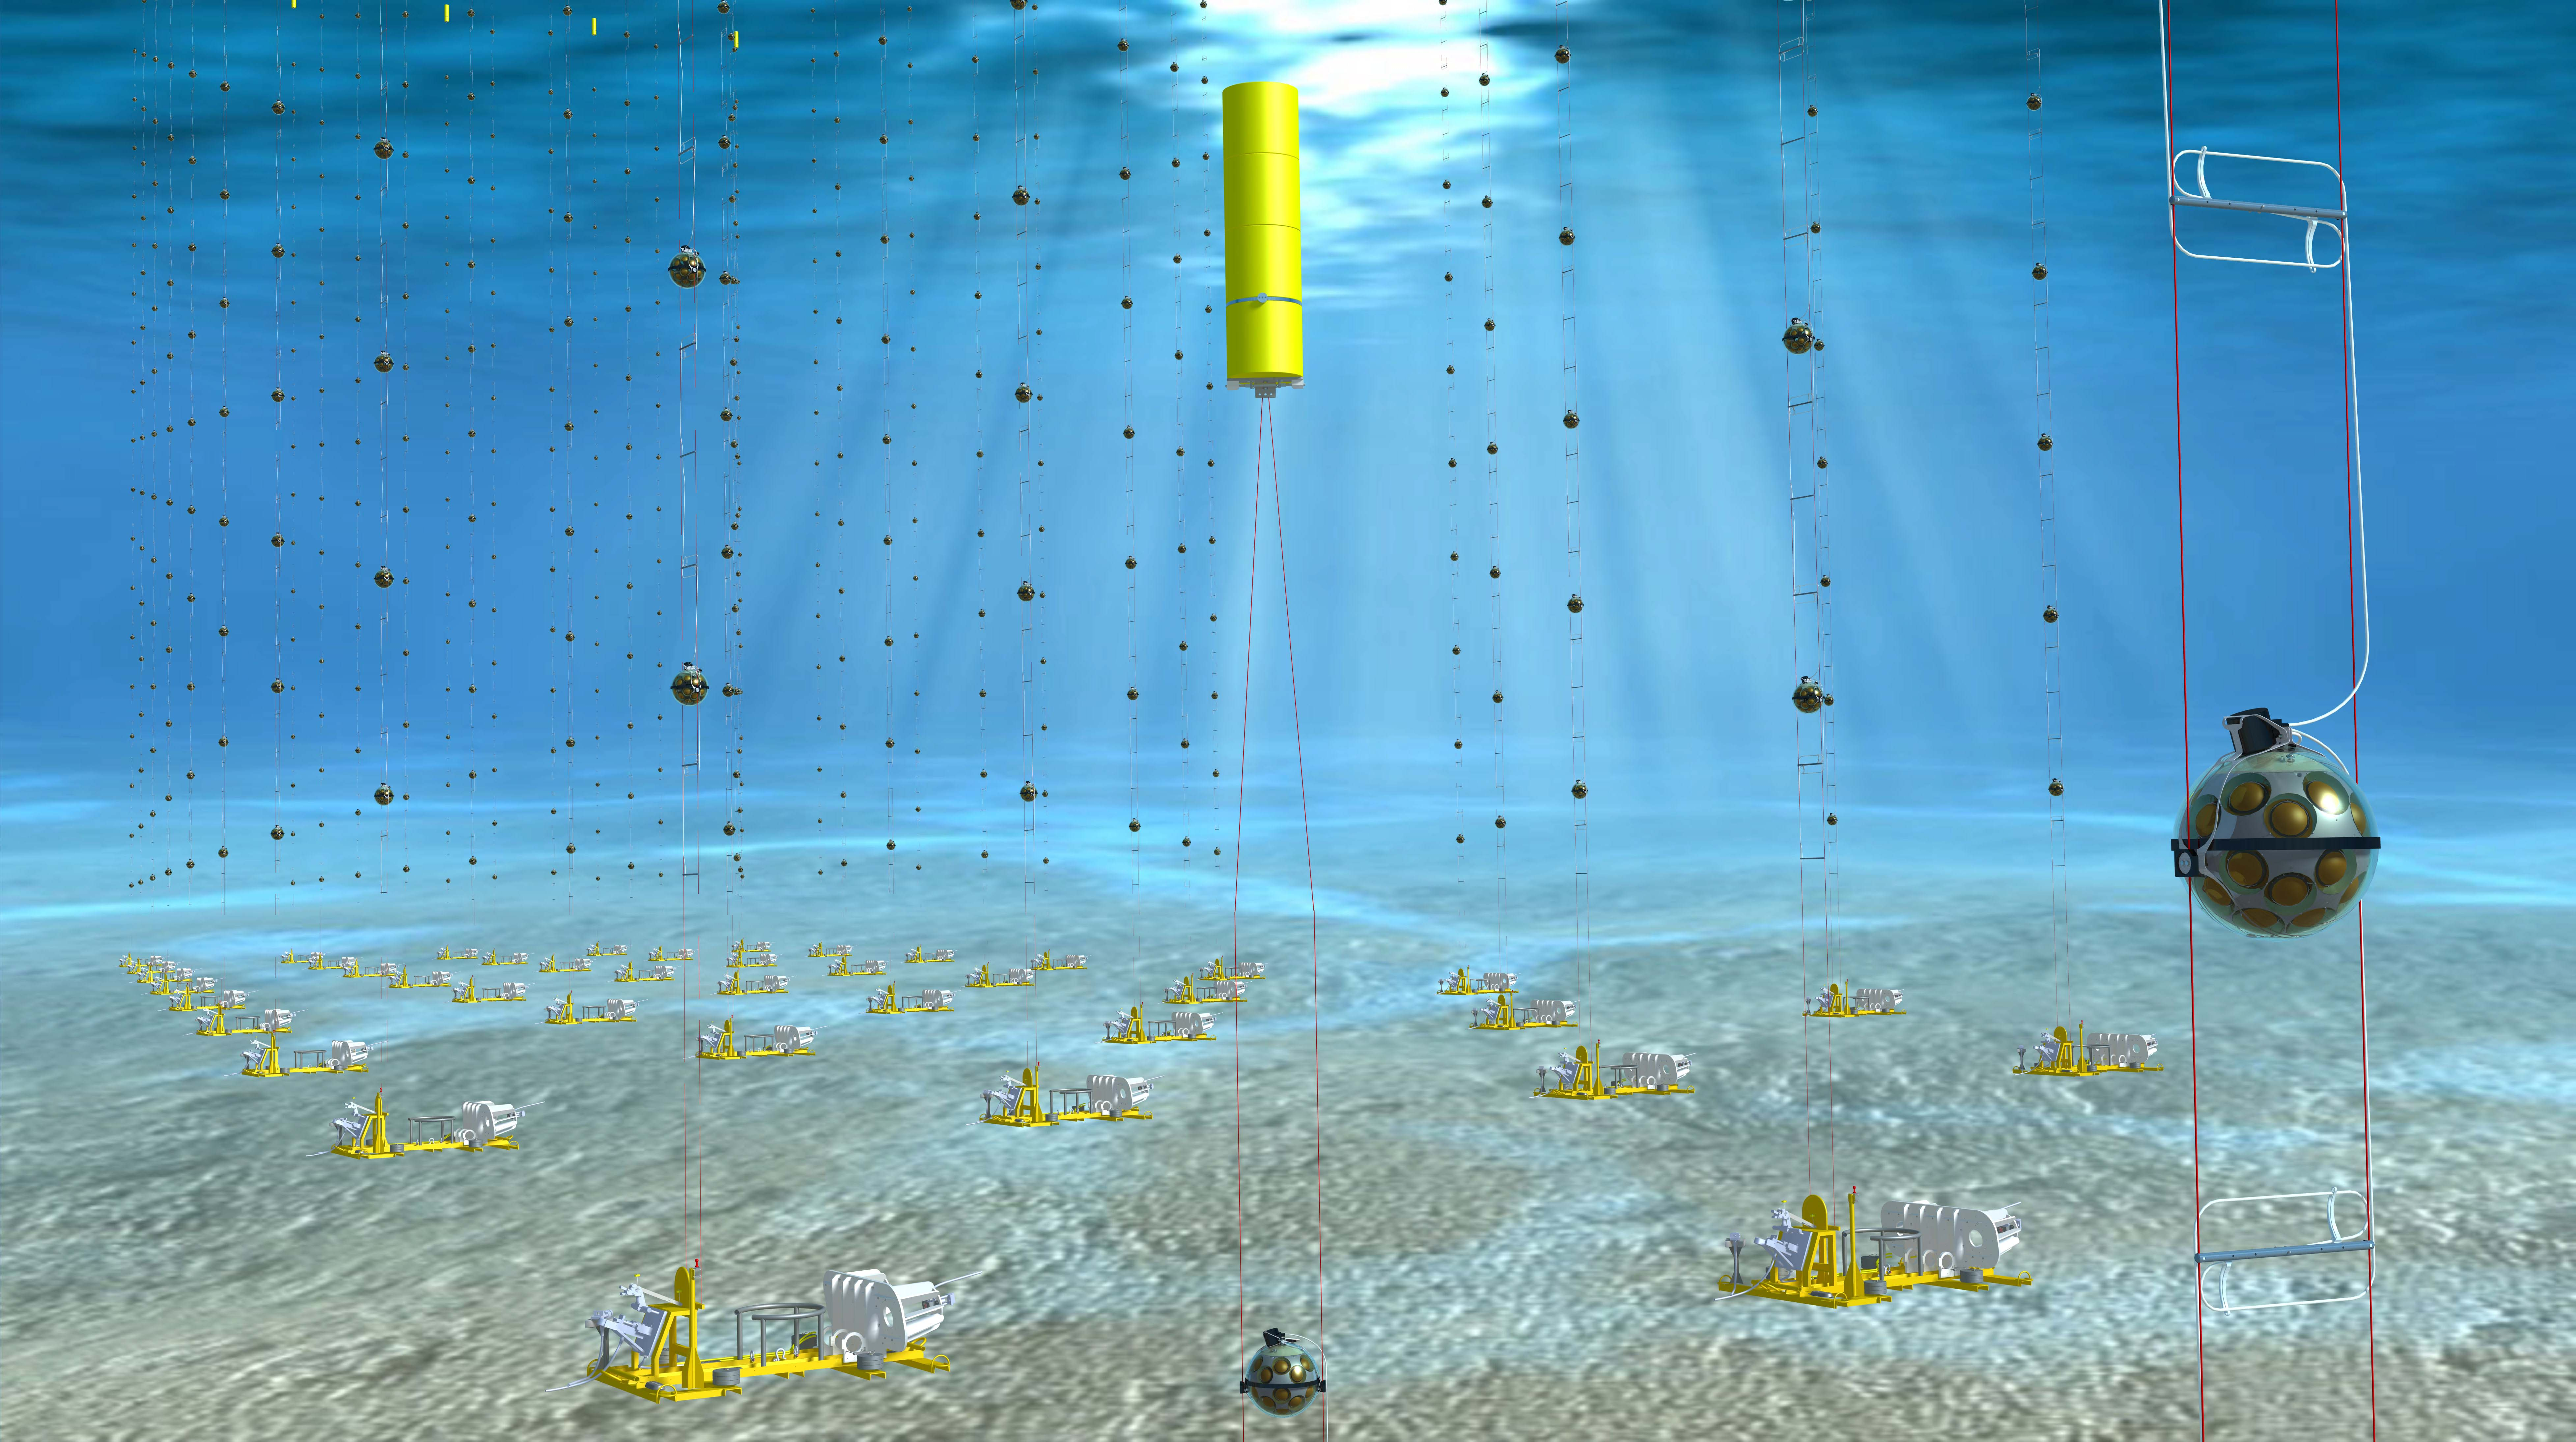
\includegraphics[width=\linewidth]{blocks.jpg}
    \caption{Artist's impression of the ARCA detector \textit{source: https://www.km3net.org}}%
    \label{fig:blocks}    
  \end{minipage}
  \begin{minipage}{0.24\textwidth}
    \includegraphics[width=\linewidth]{doms.png}
    \caption{An optical detector (DOM) \textit{source: https://www.km3net.org}}%
    \label{fig:doms}    
  \end{minipage}
\end{figure}

\section{Situation of Concern}
\label{sec:soc}

The ARCA telescope comprises of two ``blocks'' with a total volume of
$1km^{3}$. Each block consists of 115 spherical detector units (DOMs)
and each DOM consists of 31 Photo Multiplier Tubes (PMTs) in various
spatial arrangement. Figure \ref{fig:blocks} shows an artist's
impression of ARCA and figure \ref{fig:doms} depicts a DOM along with
the PMTs inside it. The PMTs are highly sensitive to light (photons),
and thus are used to detect the Cherenkov Radiation emitted from the
neutrino particle interactions. All hits are recorded by the PMTs in
the form of analog signals and those above a certain threshold are
digitized. The digital signals from all PMTs are arranged in 100ms
``timeslices'' and sent to the on-shore facility for further
processing \cite{aiello2019km3net}.

Unfortunately, there are several sources of noise like
bioluminescense, decay of Potassium 40 ($^{40}K$) and atmospheric
Muons \cite{post2019km3nnet}. Due to the high level of noise, data is
generated at an extremely high rate of 25GB/sec
\cite{adrian2016letter} and must be filtered and selectively stored
for further analysis. The state of the art for this task are known as
``Event Trigger'' algorithms \cite{adrian2016letter,aiello2019km3net}
which can filter timeslices containing just noise thus only allowing
important timeslices containing neutrino hits to pass through. The
existing event trigger algorithms namely \emph{L1} and \emph{L2}
although able to conduct the filtration in near real time, lack the
ability to do so with high accuracy thus often failing to save
important timeslices \cite{karas2019data}. Efforts have already been
made to improve the existing event trigger algorithms. Karas et al.
(2019) proposed and implemented a GPU powered pipeline which utilizes
correlation and graph community detection to identify time slices that
may contain neutrino hits whilst Post et al. (2019) suggest an
alternate using convolutional neural networks.

\section{User Requirements}
\label{sec:user-req}

The primary users of ARCA are researchers who want to study high
energy particles from outer space. The stakeholders are all member
institutes involved in the project and by extension all scientists
from these institutes who will be working with the data collected. The
requirements of the primary users and stakeholders with respect to the
data acquisition pipeline are as follows.

\begin{enumerate}
  \item[\textbf{UR1}.]\textbf{The accuracy of filtration must be extremely high.}

    Time slices which are deemed important by event trigger algorithms
    are stored for further analysis and research. Failure to store
    timeslices containing information from neutrino events can lead to
    loss of important data and hinder new discovery. Since majority of
    the data generated is noise, the pipeline must be able to prevent
    storage of unnecessary timeslices containing only noise in the
    on-shore facility.

  \item[\textbf{UR2}.] \textbf{Filtration should occur in real time.}

    The state of the art event trigger algorithms are able to process
    data in real time. The proposed alternative should be able to
    provide better data filtration quality whilst maintaining or
    improving upon its predecessor's runtime performance.

\end{enumerate}

\section{Research Question}
\label{sec:rqs}

This report presents research to improve upon the GPU Pipeline
proposed by Karas et al. (2019) to combat the limitations of the L1
and L2 event trigger algorithms. Specifically this project seeks to
answer the following research questions.

\begin{enumerate}
  \item[\textbf{RQ1}.] \textbf{Can the existing GPU pipeline be improved using Neural Networks?}

    Improvement may be achieved by reducing the processing time of the
    pipeline or improving the accuracy with which relevant timeslices
    are identified. This project focuses on achieving improvement via
    accuracy. The task of validating the runtime performance of the
    methods proposed in this paper is left to a separate project. In
    order to answer \textbf{RQ1}, the following additional questions
    are formulated.

  \item[\textbf{RQ2.}] \textbf{Can the \emph{Hit Correlation Step} be replaced with a Multi Layer Perceptron?}

    The first step of the GPU Pipeline is the Hit Correlation Step. A
    novel trigger criterion was proposed which when given a pair of
    points, can quantify their level of correlation with an accuracy
    of 80\%. The first phase of this project focuses on exploring an
    improvement to this trigger criterion using a Multi Layer
    Perceptron (MLP).
    
  \item[\textbf{RQ3.}] \textbf{Can the \emph{Graph Community Detection Step} be replaced with a Graph Convolusional Neural Network?}

    The output of the Hit Correlation Step is used to create a graph
    structure where hits from neutrino and noise are represented as
    nodes connected with an undirected edge carrying the probability
    of correlation as its weight. The Constant Potts clustering
    algorithm, which operates on the principles of Graph Community
    Detection \cite{fortunato2010community}, was used to separate the
    graph into communities of neutrino and noise hits. The second
    phase of this project focuses on achieving a better accuracy for
    clustering neutrino and noise hits into separate communities in a
    given timeslice using Graph Convolusional Neural Networks
    \cite{kipf2016semi}.
\end{enumerate}

The following chapters present the research efforts carried out to
improve The GPU Pipeline using Artificial Neural Networks. In Chapter
\ref{cha:data}, the steps taken to prepare the dataset is presented
followed by its statistical analysis and visual exploration. Since
this research initiative is based on the seminal work conducted by
Karas et al. (2019), an overview of the GPU Pipeline is presented in
Chapter \ref{cha:related-work} in addition to other related projects.
Chapters \ref{cha:mlp} and \ref{cha:gcn} present detailed analysis of
the neural networks created to replace segments of The GPU Pipeline.
Drawing from the results of the replacement models, practical
recommendations and directions for further research are laid out in
Chapter \ref{cha:rec}.

This report is intended for the primary users of ARCA with the hope to
aid in the development of the successor to the state of the art event
trigger algorithms. The report may also be used by deep learning
practitioners working in the field of neutrino detection. This report
assumes the reader posses a background in Computer Science or
Artificial Intelligence and thus is familiar with concepts such as
statistics, linear algebra and optimization. The reader is expected to
have basic understanding of the guiding principals of Deep Learning
such as Feed-Forward Neural Networks, backpropagation, binary
classification and model evaluation metrics.

\chapter{The Karas Pipeline}
\label{cha:karas-pipeline}

This chapter presents the GPU pipeline proposed by
\cite{karas2019data} (henceforth referred to as the \textit{Karas
  Pipeline} in more detail since the work presented in this report is
directly based off of this seminal work. The chapter concludes by
presenting the limitations of the Karas Pipeline and derives
motivations for a better alternative as presented in the following
chapters (see chapters \ref{cha:pm} and \ref{cha:gcd}).

\citeauthor{karas2019data} presents a data processing pipeline to filter
timeslices containing hits from neutrino events from those containing only
noise. The pipeline is able to achieve this filtration by processing the data
in 3 steps, described in more detail below.

The first step of The Karas pipeline is the Hit Correlation step. In this
step, pairs of hits (from events and noise) are considered and the correlation
along two axes namely space and time are
considered. \citeauthor{karas2019data} proposes \textit{The Pattern Matrix
Criterion (PMC)}. The PMC operates by creating a correlation criterion based
on the probability that a given space and time difference occurs between two
event hits. From domain knowledge, the evaluation is limited to 100m and 300ns
for space and time differences respectively. The algorithm is evaluated with
a dataset containing 130 event hits and 5000 noise hits and scores in the
range of 0.3 - 0.375 is reported for the recall, precision and F1 metrics
and an accuracy of 80\% is achieved.

The second step of the Karas pipeline is the Graph Community Detection
step. The Constant Potts Model (CPM) is used to group event and noise hits
(represented as nodes of a graph) into separate communities (or clusters)
based on the density of connections and the size of the communities. The
output of the PMC is utilized to connect causally related nodes with an
undirected edge and the probability of correlation is assigned as the weight
of the edge. The model is tested using a dataset consisting of 130 event hits
and 5000 noise hits. The model is able to perform exceptionally well and
groups most event hits into a single community and the noise in another. No
performance metrics are reported however.

The third and final step of the pipeline is the Classification step. The two
parameters namely the Probability Threshold (PT) of the PMC and the $\gamma$
of the GCD step are experimented with to determine the optimal thresholds. All
hits above the specified thresholds are classified as event hits the rest are
classified as noise.

\subsection{Limitations of the Karas Pipeline}
\label{sec:karas-pipeline-limitations}

% limitation: edges are only assigned to nodes which are deemed to be related
% by the PMC, since the probability threshold is manually set, some event hits
% may get classified as noise
% limitation: the communities are created by looking at the density of
% connections and size of communities, some really small event communities may
% get overlooked

% step 3: classification step
% - tested with 1,000,000 hits; ~7000 event hits and the rest noise
% - based on output of the GCD step, timeslices with event communities are
%   classified as important and the rest not important
% - experiments with the PT and \gamma parameters are done to determine the
% optimal model
% - communities above the PM and \gamma thresholds are considered to be event
%   hits and the rest noise
% limitation: unable to classify communities of size smaller than 20 hits

The Karas Pipeline is able to identify timeslices with neutrino event
hits more accurately compared to its predecessors such as the L1 and
the L2 filtration. However, the pipeline still has certain limitations
which hinders its performance, thus motivating a need for a better
alternative.

To begin, the space and time difference based on which the PMC
determines if two hits are causally related to one another, is static.
This results in event hits which do not meet these thresholds to be
incorrectly given a low probability of correlation to its sibling
(related) hits.

The performance of the GCD step directly depends on the output of the
PMC since the edges between causally related nodes and the weight it
carries is determined from the PMC. Thus, any limitations of the PMC
cascade down into the GCD and by extension, also into the
classification step.

% the PT is static, this may incorrectly classify event hits as noise

The CPM creates communities by observing the density of connections
and the size of the communities. These thresholds are once again
static which results in small communities being overlooked.

Finally, the classification step also operates on static values of the
PT and $\gamma$ and thus is unable to identify communities of size
smaller than 20 hits.

% this file is called up by thesis.tex
% content in this file will be fed into the main document

\chapter{Data Preparation} % top level followed by section, subsection
\label{cha:data-prep}

% ----------------------- contents from here ------------------------

At the time of undertaking this project, the KM3NeT Neutrino Telescope was
still under construction, thus  simulated data provided by Nikhef was used for
the project. The data itself was split onto two parts namely \emph{events} and
\emph{noise}, both of which came from different sources and in different
formats.

\section{Preparation of \emph{events} dataset}%
\label{sec:data-prep-events}
The \emph{events} dataset was provided as a \emph{HDF5} (Hierarchical Data
Format) with a size of 42MB consisting of the \texttt{/data/mc\_hits} and
\texttt{/data/mc\_info} tables. For the purposes of this project, the two
tables were combined such that each row in the \textit{mc\_hits} table contains
it's corresponding 'event\_id' from the \textit{mc\_info}
table. A \texttt{label} column was added containing a value of '1' and the
resulting table (henceforth referred to as the \emph{events} dataset) was saved as
a CSV file for future use.

\section{Preparation of \emph{noise} dataset}%
\label{sec:data-prep-noise}
The \emph{noise} data was generated using a Python library written and
maintained by Nikhef, \texttt{k40gen}.
\texttt{k40gen.Generators(21341, 1245, [7000., 700., 70., 0.])} was
used to create an instance of a generator where the first two
arguments are random seeds followed by a list of rates at which
single, double, triple and quadruple hits should be generated. The
generator instance is then passed into \texttt{k40gen.generate\_40()}
method which returns a (4, n) array containing (time (t), dom\_id,
pmt\_id, time over threshold (tot)). The position coordinates (ie.
\texttt{x}, \texttt{y}, \texttt{z} coordinates) for each datapoint was
provided in a \emph{positions.detx} file which was parsed using the
Numpy Python package \cite{numpy} and added to the \emph{noise} array.
The Python library Pandas \cite{pandas} was used to convert the array
into a (n, 4) dataframe. A \texttt{label} column was added containing
a value of '0' and the dataframe was saved as a 3.9GB CSV file.

\section{Preparation of \emph{main} dataset}%
\label{sec:data-prep-main}

To create the \emph{main} dataset for the project, the \emph{events} and
\emph{noise} datasets were combined. Both datasets were read into memory as
Pandas dataframes and their columns were renamed consistently. The two
dataframes were concatenated and sorted based on the \texttt{time} column. Rows
with a negative \texttt{time} value were dropped along with columns which are
not relevant to this project. The \texttt{time} column was discretized into
15000ns bins and the resulting values were added to the \texttt{timeslice}
column. The resulting dataframe was saved as a 1.9GB CSV file.

% ---------------------------------------------------------------------------
% ----------------------- end of thesis sub-document ------------------------
% ---------------------------------------------------------------------------

% this file is called up by thesis.tex
% content in this file will be fed into the main document

\chapter{Data Exploration} % top level followed by section, subsection
\label{cha:data-exp}

% ----------------------- contents from here ------------------------

The \emph{main} dataset (generated as per the steps outlined in Chapter
\ref{cha:data-prep}) was explored using statistical analysis and
visualizations to observe any patterns and "local trends" that may be
present. The following chapter presents the analysis that were done and the
observations made.

Note that a random sample of only 10\% of the data was taken for the following
visualizations. This is because it is difficult to draw reasonable conclusions
from the plots due to the high number of data points when the entire dataset is
used.

\section{Descriptive Statistics}%
\label{sec:data-exp-desc-stats}

\begin{table}[h]
  \centering
  \caption{Description of columns}
  \label{tab:desc-cols}
  \begin{tabular}{p{1.5cm}p{1.5cm}p{2cm}p{8cm}}
    \hline
    Column & Data type & Unit & Description \\
    \hline
    x, y, z & float & meters (m) & The position within the detector where the hit was detected, they represent the x,y,z coordinates of the hit respectively. \\
    t & float & nano seconds (ns) & The time at which the hit was detected. \\
    label & int & NA & The type of hit, '0' represents noise and '1' represents a neutrino hit \\
    event\_id & int & NA & The id of the event to which the hit is related to. The id itself does not have any meaning, it is simply used to identify hits that originated from the same event. \\
    timeslice & int & NA & The id of the timeslice to which the hit belongs. The id itself does not have any meaning, it is simply used to group hits into discrete bins. \\
    \hline
  \end{tabular}
\end{table}

Table \ref{tab:desc-stats} presents the descriptive statistics of the
\emph{main} dataset. The dataset consists of 7 columns and roughly 4.5 million
rows, Table \ref{tab:desc-cols} provides more information on the columns on the
dataset. The dataset does not contain any \texttt{nan} or \texttt{null} values
except for the \texttt{event\_id} column where rows containing noise hits are
not associated with any event.

\begin{wrapfigure}{r}{0.5\textwidth}
  \centering
  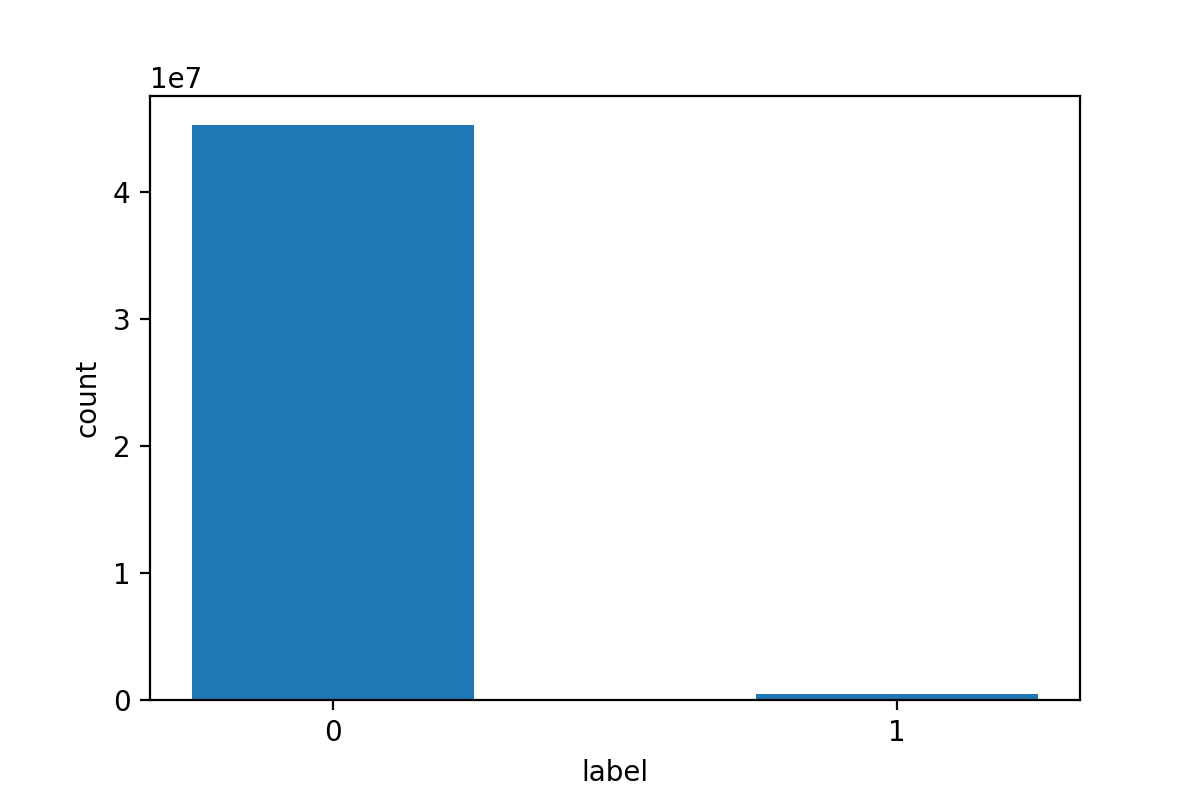
\includegraphics[width=0.9\linewidth]{dist-label.png}
  \caption{Distribution of \texttt{label} column}%
  \label{fig:dist-label}
\end{wrapfigure}

Next, the correlations amongst features is checked, the "Pearson"
correlation is used. Figure \ref{fig:corr} represents the correlation
matrix of all features. No significant correlations are observed
between \texttt{x}, \texttt{y}, \texttt{z} and \texttt{t} which
indicates that ML models may not be able to learn anything from the
dataset without the aid of feature engineering.

\begin{figure}[h]
  \centering
  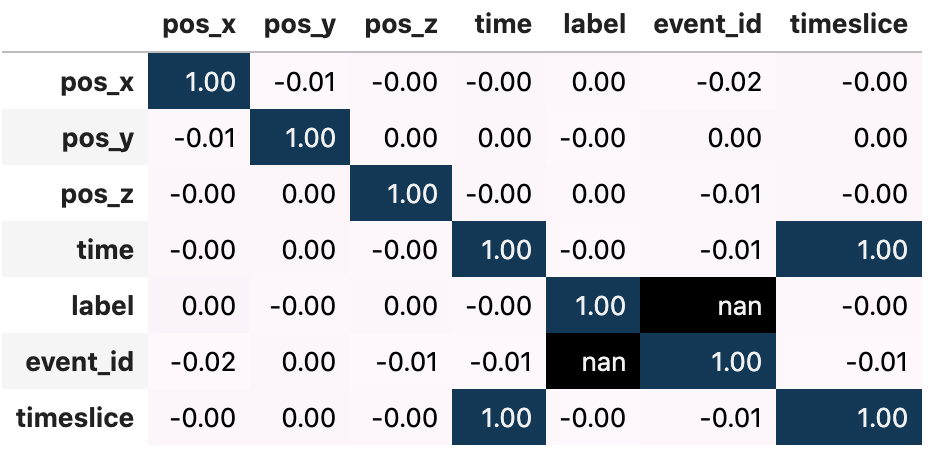
\includegraphics[width=0.8\linewidth]{correlation.png}
  \caption{Correlation matrix of features}
  \label{fig:corr}
\end{figure}

The distribution of the \texttt{label} column is presented in Figure
\ref{fig:dist-label}. A severe class imbalance is noted between events and
noise hits. To be precise, the dataset contains 489906 instances of events
compared to over 4.5 million instances of noise. An effective strategy to
handle the class imbalance will need to be devised during training of models
to prevent the model from overfitting.

\begin{table}[t]
  \centering
  \caption{Descriptive statistics}
  \label{tab:desc-stats}
  \begin{tabular}{lrrrrrrr}
    \hline
          & x & y & z & t & label & event\_id & timeslice \\
    \hline
    count & 4.58e+7 &  4.58e+7 &  4.58e+7 &  4.58e+7 &  4.58e+7 &  489906 &  4.58e+7 \\
    mean  & 1.16e-02 & -1.59e-02 &  1.17e+02 &  5.00e+07 &  1.06e-02 &    2862.00 &  3.33e+03 \\
    std   & 5.12e+01 &  6.22e+01 &  4.86e+01 &  2.89e+07 &  1.02e-01 &    1667.61 &  1.92e+03 \\
    min   & -9.46e+01 & -1.15e+02 &  3.77e+01 &  0.00e+00 &  0.00e+00 &       0.00 &  0.00e+00 \\
    25\%  & -4.50e+01 & -5.79e+01 &  7.40e+01 &  2.50e+07 &  0.00e+00 &    1392.25 &  1.66e+03 \\
    50\%  & 1.30e+00 & -4.18e+00 &  1.21e+02 &  5.00e+07 &  0.00e+00 &    2887.00 &  3.33000e+03 \\
    75\%  & 4.04e+01 &  4.85e+01 &  1.60e+02 &  7.50e+07 &  0.00e+00 &    4304.75 &  5.00000e+03 \\
    max  & 9.62e+01 &  1.05e+02 &  1.96e+02 &  1.01e+08 &  1.00e+00 &    5734.00 &  6.77e+03 \\
    \hline
  \end{tabular}
\end{table}

\section{Verification of Bias}%
\label{sec:data-exp-verification-bias}

The \emph{events} dataset is synthetically generated using simulations. As such,
it is likely that the event hits in each timeslice may occur at a specific
time such as at the beginning, middle or end of the timeslice. Having such
a pattern in the dataset may bias the model since it may learn this pattern and
thus fail to generalize. If this pattern does exist in the dataset, corrective
measures need to be taken such that the event hits in each timeslice are
uniformly distributed.

To verify the existence of such patterns in the dataset, the mean time
of event hits across all events was visualized as a scatter plot as
depicted by Figure \ref{fig:bias-verification}. A uniform distribution
is noted with no visible patterns. Thus no bias exists in the dataset
and it is deemed suitable for further analysis.

\begin{wrapfigure}{l}{0.5\textwidth}
  \centering
  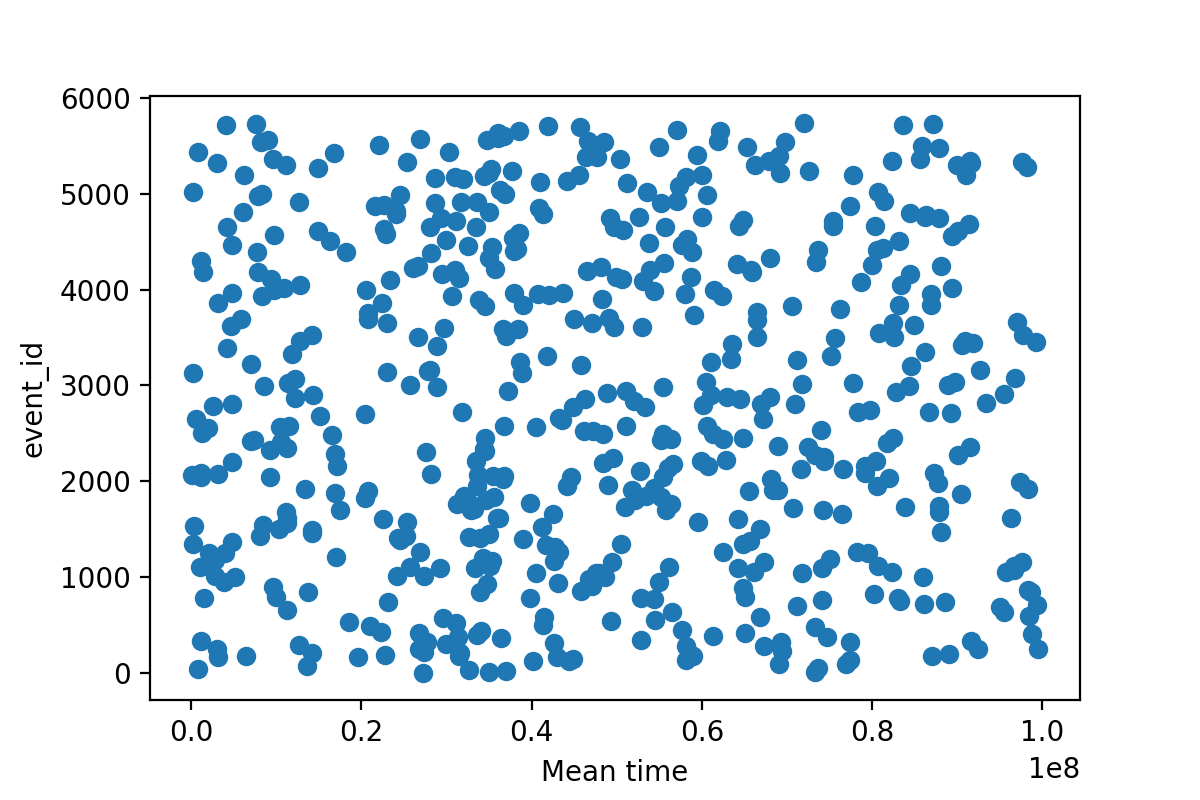
\includegraphics[width=0.9\linewidth]{bias-verification.png}
  \caption{Verification of Bias}%
  \label{fig:bias-verification}
\end{wrapfigure}

\section{Exploration of Interesting Timeslices}%
\label{sec:data-exp-interesting-timeslices}

Figure \ref{fig:dist-hits-per-timeslice} represents to total number of
event hits per timeslice. The dataset is discretized into 6759
timeslices of which 2783 timeslices contain only noise hits. This is
corroborated by Figure \ref{fig:dist-hits-per-timeslice} which
presents a skewed distribution where many timeslices contain few to no
event hits and few timeslices contain a high number of event hits.

\begin{wrapfigure}{r}{0.5\textwidth}
  \centering
  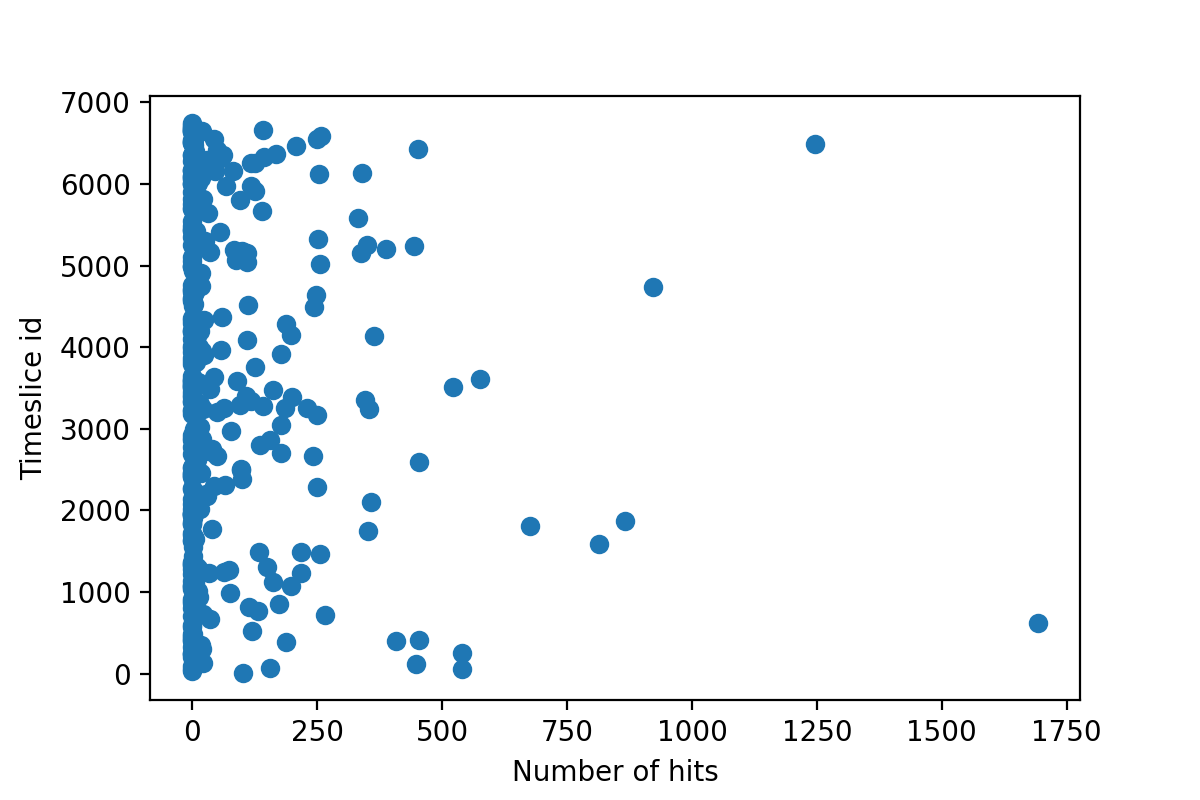
\includegraphics[width=0.9\linewidth]{dist-hits-per-timeslice.png}
  \caption{Distribution of event hits per timeslice}%
  \label{fig:dist-hits-per-timeslice}
\end{wrapfigure}

Figure \ref{fig:dist-timeslice-largest} depicts a scatter plot of
\emph{timeslice 615} which contains the largest number of event hits.
It is observed that event hits occur close to each other in space and
time (represented by the yellow, blue and green points) whilst
background hits are uniformly distributed in space and time
(represented by the purple points).

\begin{figure}[h]
  \centering
  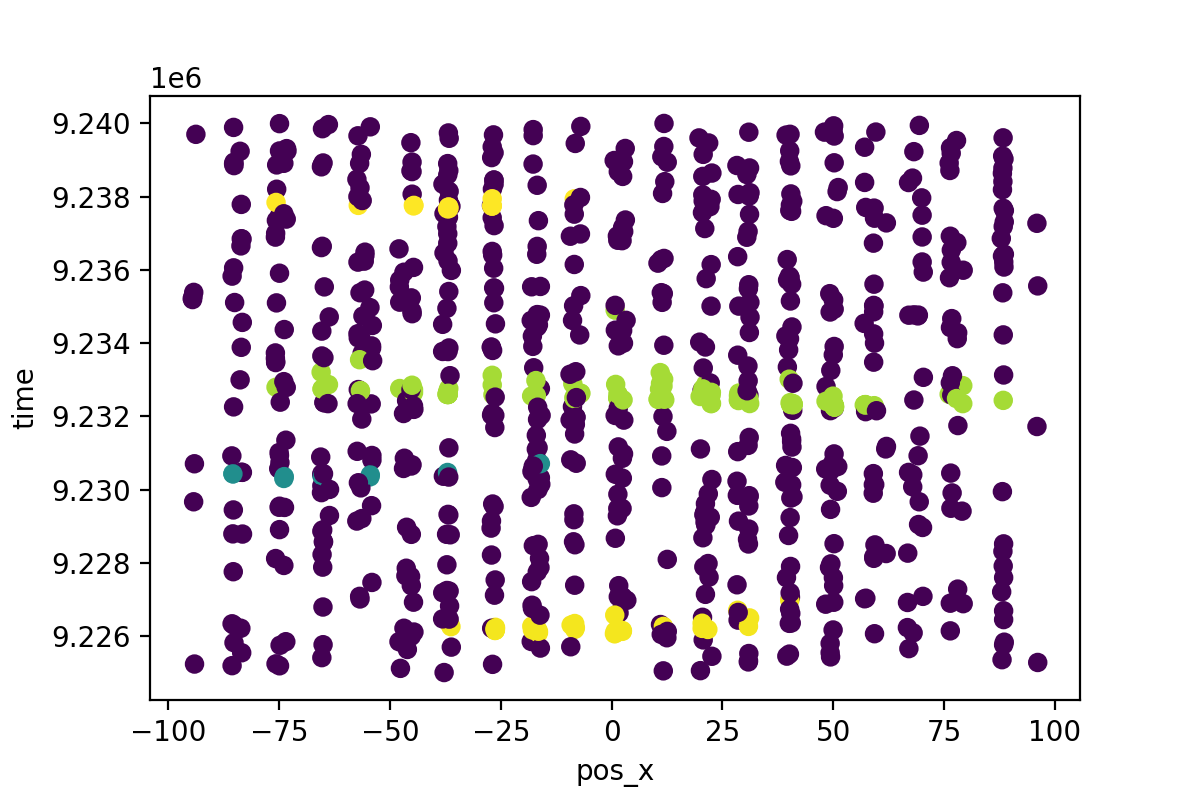
\includegraphics[width=0.9\linewidth]{dist-timeslice-largest-posx-time-eventid.png}
  \caption{Distribution of Timeslice 615}%
  \label{fig:dist-timeslice-largest}
\end{figure}


% ---------------------------------------------------------------------------
% ----------------------- end of thesis sub-document ------------------------
% ---------------------------------------------------------------------------

% this file is called up by thesis.tex
% content in this file will be fed into the main document

\chapter{Replacement for Hit Correlation Step} % top level followed by
% section, subsection
\label{cha:mlp}

% ----------------------- contents from here ------------------------
% 
This chapter presents the replacement created using a Multi Layered
Perceptron (MLP) for the \textit{Hit Correlation Step} of the Karas
pipeline (see \ref{cha:karas-pipeline}). It is observed that a MLP is
able to identify causally related hits with a higher accuracy,
precision and recall compared to the PMC. The chapter begins by
explaining how the data is created followed by its visual examination.
The training and testing procedure for the model is explained next.
The chapter concludes with discussions of the experiment results and
next steps.

\section{Data Preparation}
\label{sec:mlp-data-prep}

% TODO find the mathematical term for the series, could be n^{2}-n!
Figure \ref{fig:mlp-data} summarizes the MLP dataset creation process.
With an input data of shape $(n, 4)$ (\emph{n} rows and 4 columns
representing \emph{x, y, z, and t}), an output data of shape
\texttt{($\sum_{k=n-1}^{1}k$, 9)} is obtained. A significant rise in
the number of rows is observed since each row (representing a single
hit) is paired with all rows that follow. The output dataset consists
of 9 columns due to the presence of \emph{x, y, z and t} columns of
two hits plus the label column.

\begin{figure}[htb]
  \centering
  \begin{minipage}[t]{0.74\textwidth}
    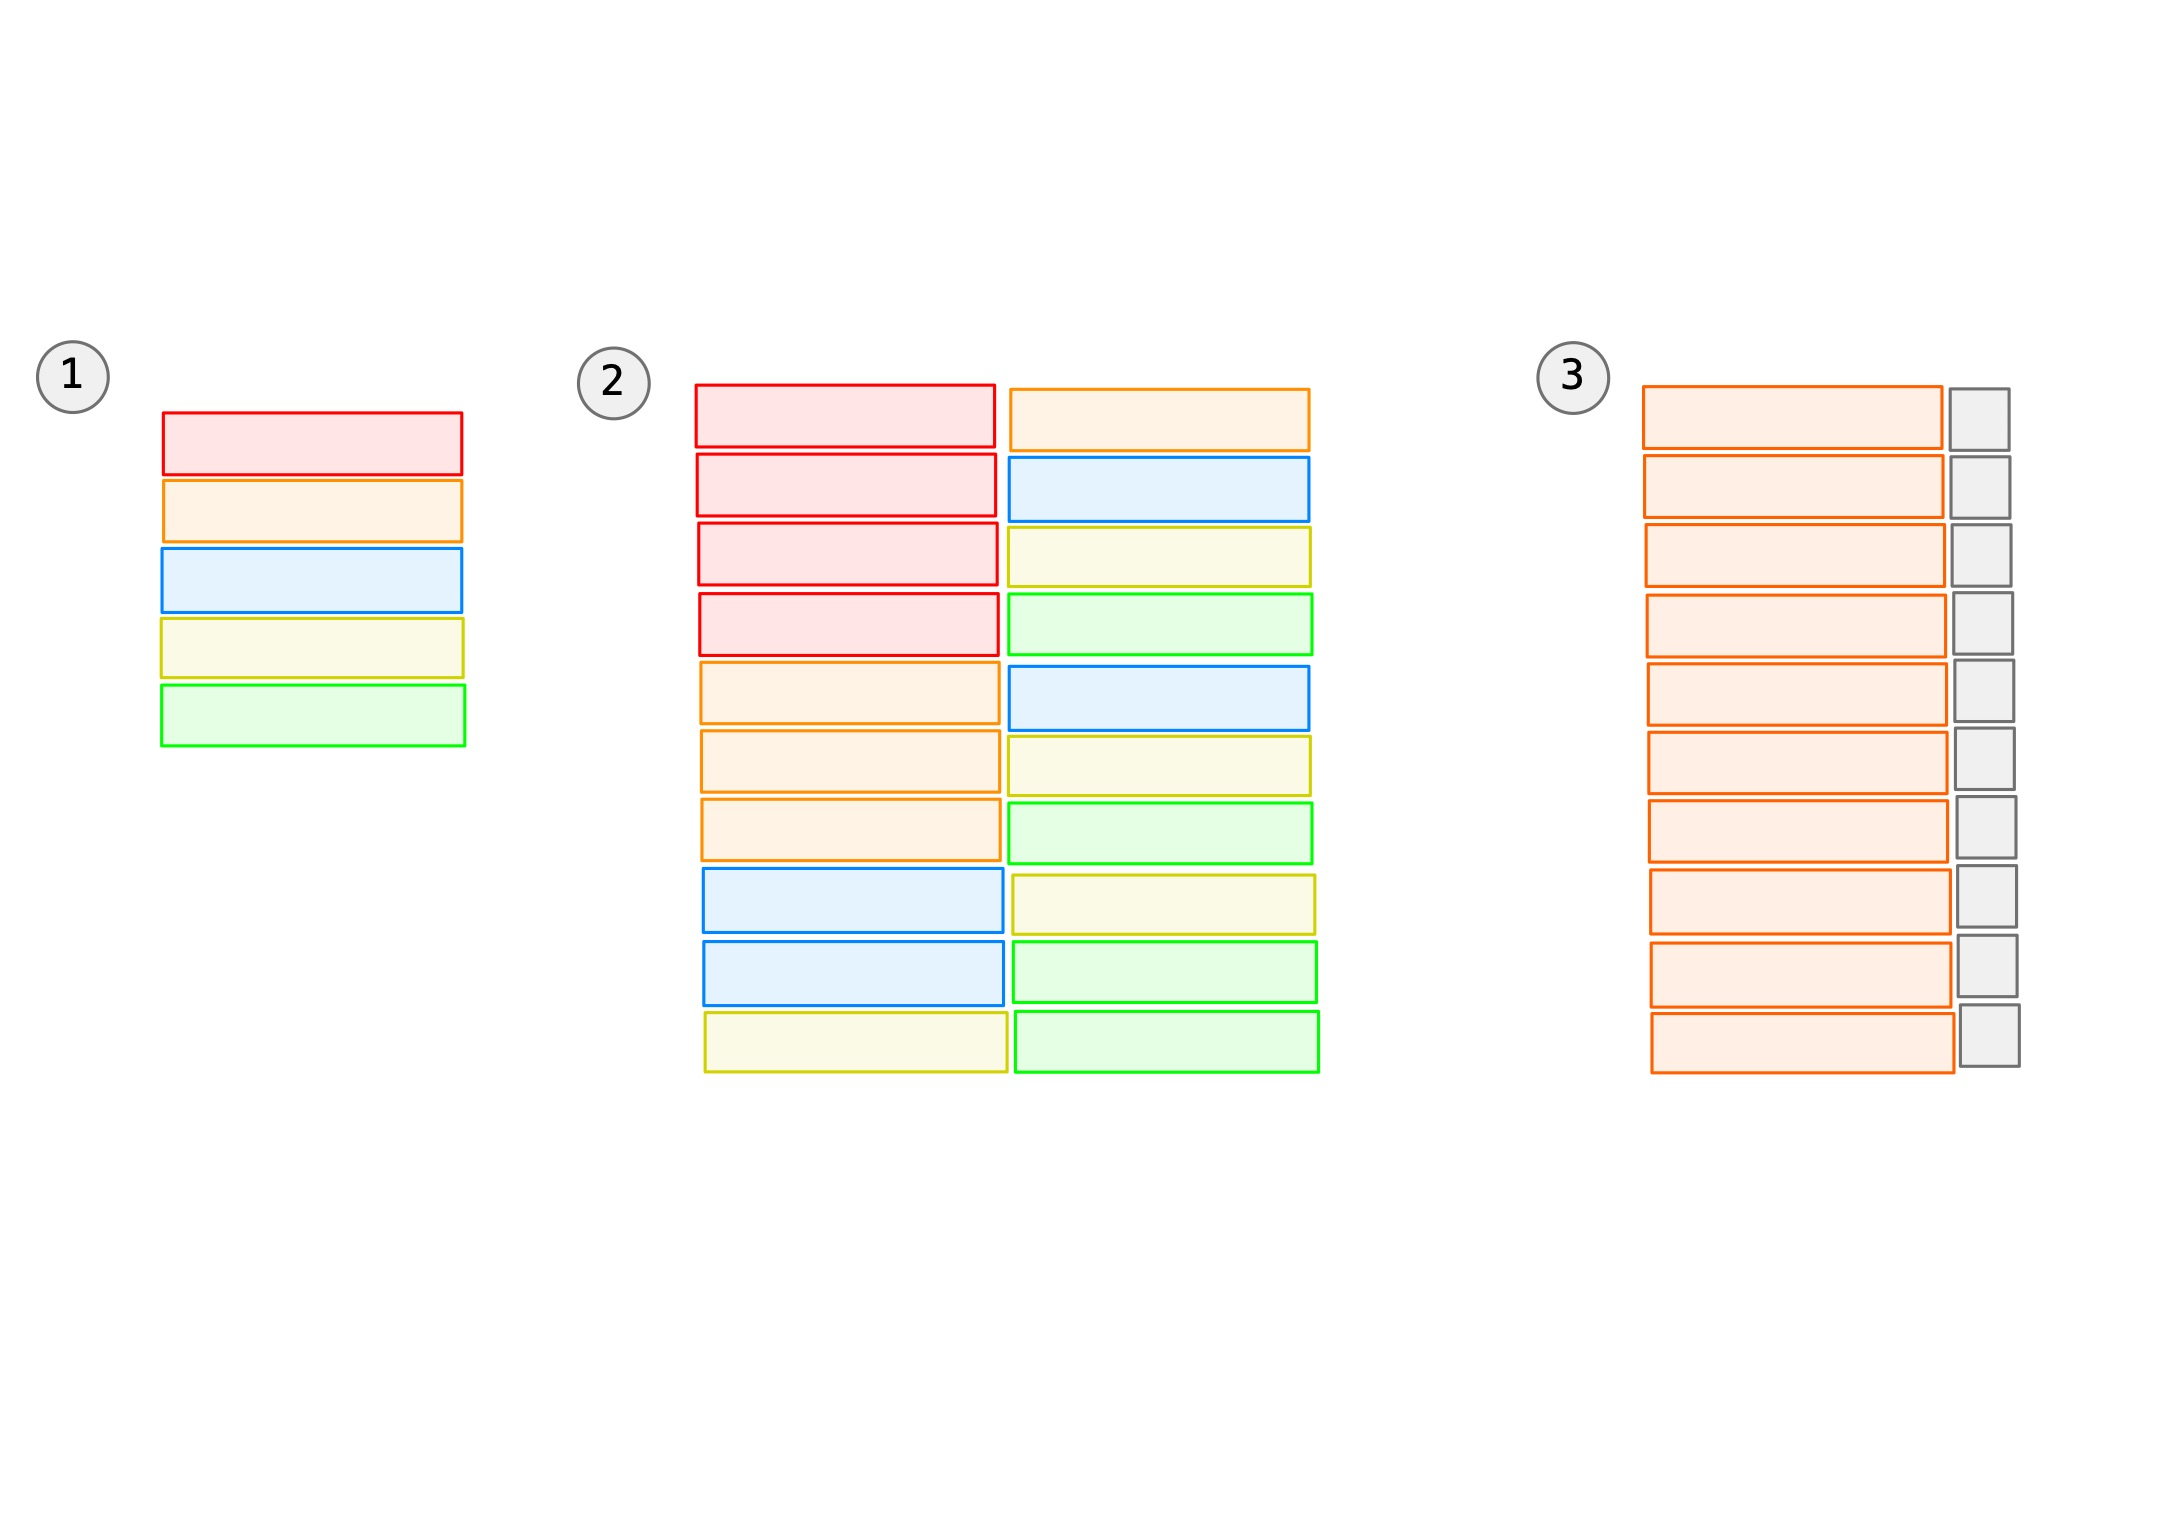
\includegraphics[width=\textwidth]{mlp-data.jpg}
    \caption{Overview of MLP dataset creation procedure. \textbf{(1)}
      The main dataset where each row represents a hit, here an example
      set containing 5 rows is shown for simplicity. \textbf{(2)} The
      MLP dataset is generated from the main dataset consisting of all
      unique pairs of hits. Algorithmically, this is done by pairing
      each hit with the subsequent hits below it as demonstrated with
      the use of colors. \textbf{(3)} The difference between the hits is
      taken (dark orange) and a label is assigned to each row (gray).}
    \label{fig:mlp-data}
  \end{minipage}
  \begin{minipage}[t]{0.24\textwidth}
    \centering
    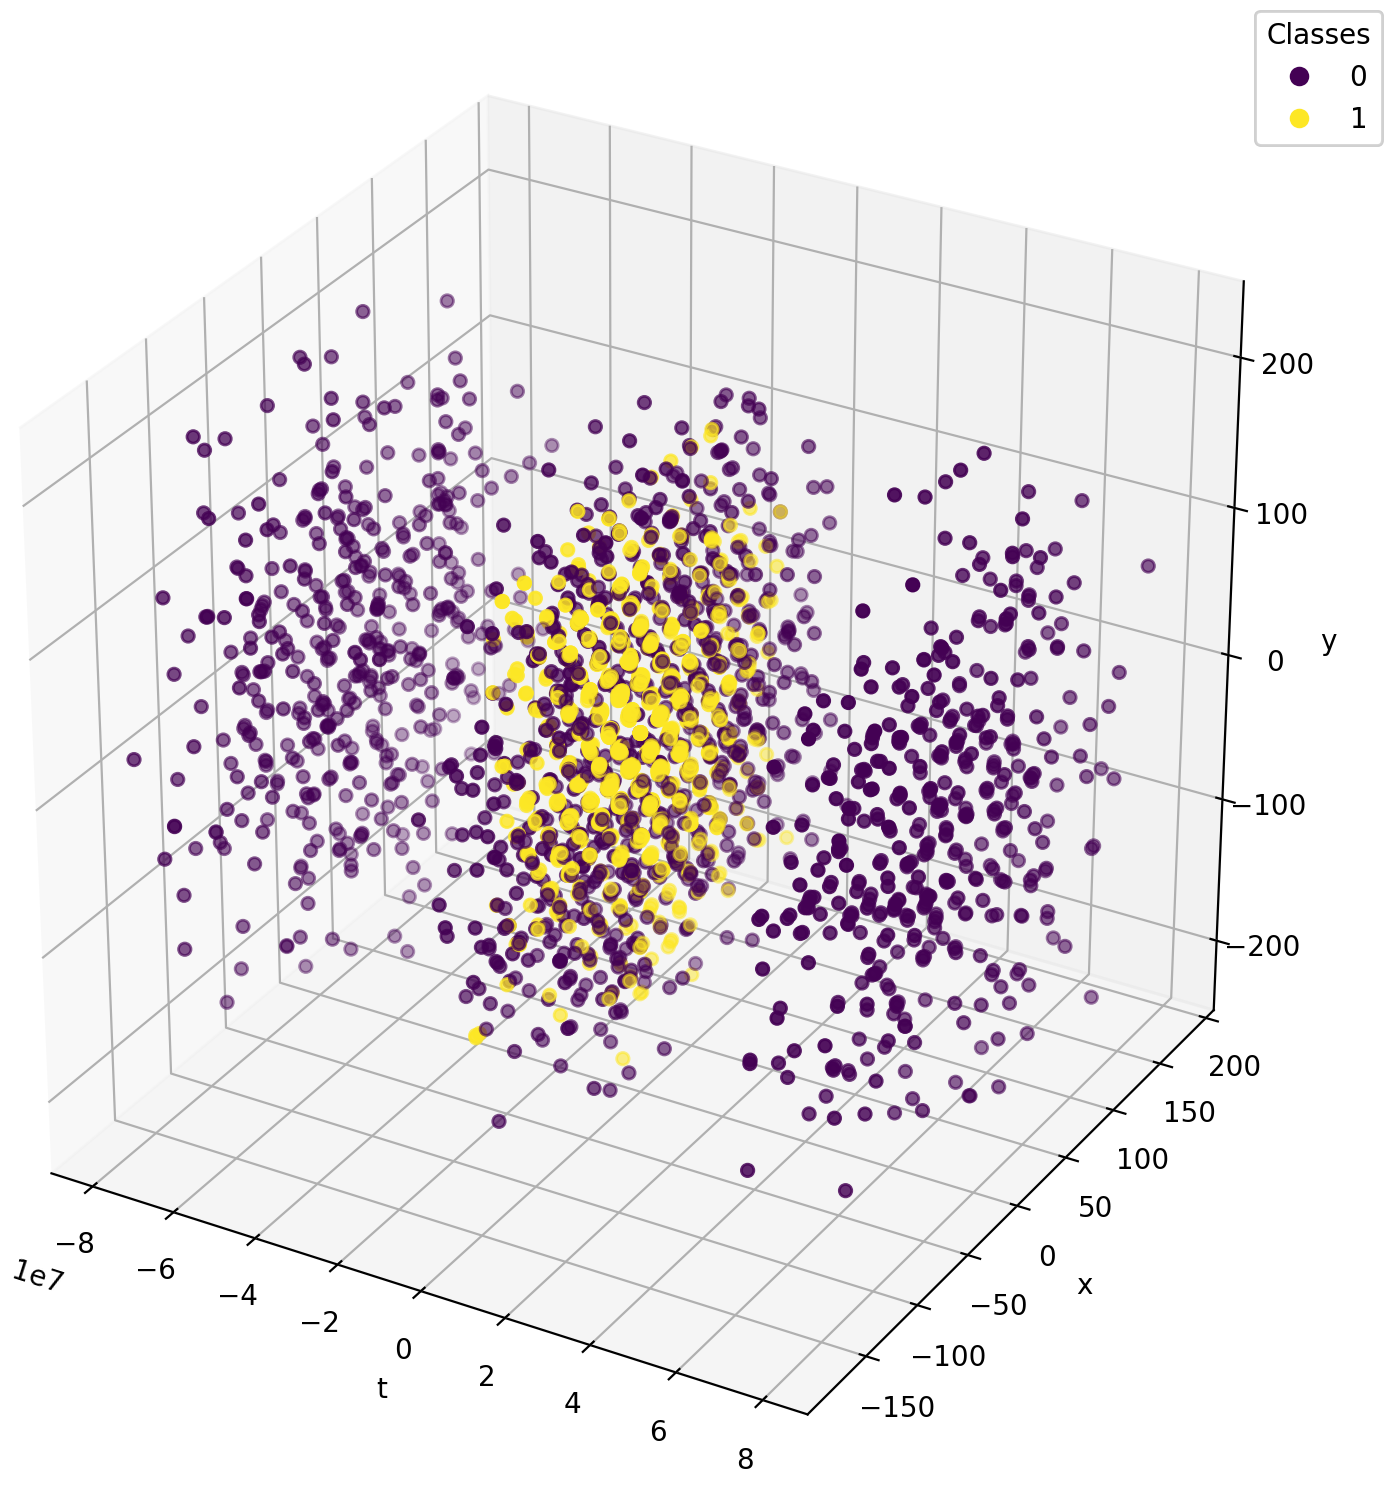
\includegraphics[width=\linewidth]{mlp-train-dist.png}
    \caption{Distribution of MLP training dataset.}
    \label{fig:mlp-train-dist}
  \end{minipage}
\end{figure}

The label column is populated based on the values of the
\texttt{event\_id} column of the two hits. The row is assigned a label
of 1 if the two hits have the same event id, which signifies that they
originated from the same neutrino event and hence are causally related
to each other. If the event id of the two hits are not the same then
they are assigned a label of 0.

Better model performance was observed when the model was trained with
the difference between hits in time and space. As a result, the final
dataset of shape \texttt{$\sum_{k=n-1}^{1}k$, 5} was obtained. The
fist 4 columns being the difference of \emph{x, y, z and t} vectors of
the paired hits and the last column being the label. The data is
additionally scaled between $[0,1]$ as this is recommended and
empirically proven to improve model performance and prevent vanishing
gradients during training
\ref{bengio2012practical,goodfellow-et-al-2016}.

\subsection{Preparation of Training Data}
\label{sec:mlp-data-prep-train}

The main dataset is highly skewed, with the \textbf{majority or
  negative class} being hits from background noise and the
\textbf{minority or positive class} being hits from neutrino events.
Thus, the training set created is also skewed with the minority class
being related hits and majority class being unrelated hits. To
maximize the number of positive examples in the training set, a random
sample was taken from the top 5 timeslices of the main dataset with
the most number of event hits. The model is required to classify
related and unrelated hits which can be done by observing the space
and time difference between the given points. Since this phenomenon is
consistent across the entire main dataset, training using a sample
does not introduce any bias into the model.

The training set still however contains a skewed distribution of
examples, and training the model with such a dataset will result in a
model that is biased to the majority class. To combat this problem,
the majority class is \emph{undersampled} such that the number of
examples for each class is the same. Figure \ref{fig:mlp-train-dist}
shows the distribution of a random sample of the training set. It is
observed that the related hits occur close to one another in space and
time whilst the noise hits are scattered throughout which should aid
the model to learn. A fraction of the training set is kept as a hold
out or validation set to evaluate the model's training. Table
\ref{tab:mlp-train-dist} presents the distribution of the training and
validation sets.

\begin{table}[htb]
  \centering
  \caption{Distribution of MLP Training and Validation Datasets.}
  \begin{tabular}{lrrr}
    \hline
    & Total examples & Positive examples & Negative examples \\
    Training & 48,434 & 24,217 & 24,217 \\
    Validation & 23,856 & 11,928 & 11,928 \\
    \hline
  \end{tabular}
  \label{tab:mlp-train-dist}  
\end{table}

\subsection{Preparation of Testing Data}
\label{sec:mlp-data-prep-test}

Whilst the training dataset contains equal number of examples for each
class, the testing dataset maintains it's skewed distribution since
this represents realistic data which the model will be required to
classify. Four variants of the testing dataset with varying level of
examples of related hits were created as listed in Table
\ref{tab:mlp-test-dist}. In practice, the pipeline will observe
timeslices which contain no to very few related hits, thus the
performance of the model on TS1 and TS2 are of vital importance.

\begin{table}[htb]
  \centering
  \caption{Distribution of MLP Test Datasets.}
  \begin{tabular}{lrrr}
    \hline
    & Total examples & Positive examples & Negative examples \\
    \textbf{TS1} & 774,390 & -- & 774,390 \\
    \textbf{TS2} & 5,829,405 & 10 & 5,829,395 \\
    \textbf{TS3} & 5,880,735 & 1176 & 5,879,559 \\
    \textbf{TS4} & 364,231 & 8,372 & 355,859 \\
    \hline
  \end{tabular}
  \label{tab:mlp-test-dist}
\end{table}

\section{Model Description}
\label{sec:mlp-model-desc}

The expectation of the model is to identify if two given points are
causally related to each other or not. As revealed through data
exploration in Chapter \ref{cha:data-exploration}, hits originating from
neutrino events occur close to each other in space and time. Thus, The
expectation from the model is to learn this phenomenon by training
over pairs of points and classify unseen data as related or unrelated.

\begin{table}[htb]
  \centering
  \begin{tabular}{lr}
    \hline
    Loss & BCELoss \\
    Optimizer & Adam \\
    Learning rate & 0.001 \\
    Hidden activation function & ReLU\\
    Output activation function & Sigmoid \\
    Training batch size & 16 \\
    Testing batch size & 32 \\
    \hline
  \end{tabular}
  \caption{GCN Model Parameter Summary.}
  \label{tab:gcn-model-param}
\end{table}

The parameters of the model are summarized in Table
\ref{tab:mlp-model-param}. The Adam optimizer with a learning rate of
$0.001$ is used to optimize the loss function since it is considered a
reasonable start for many optimization problems and has been
empirically proven to outperform other algorithms such as
\textit{Stocastic Gradient Descent (SGD)}, \textit{RMSProp} and
\textit{Adagrad} \cite{ruder2016overview}. Being a binary
classification task, the \textit{Binary Cross Entropy Loss (BCELoss)}
(also known as \textit{Log Loss}) was selected as the loss function
since it has been established as the standard loss function for binary
classification tasks \cite{painsky2018universality}. As the BCELoss
function expects an input in the range of $[0, 1]$, the
\textit{Sigmoid} activation function was chosen for the output layer.
The \textit{ReLU} activation function was chosen for the hidden layers
since it is generally considered a good start for most problems
\cite{nwankpa2018activation, wang2019learning}. A batch size of 16 is
used for the training and validation sets whilst a larger batch size
of 32 is used for the testing set since these value are often
recommended as good defaults by machine learning practitioners
\cite{bengio2012practical,Goodfellow-et-al-2016}.

\begin{table}[htb]
  \centering
  \begin{tabular}{lrrr}
    \hline
    Layer Position & Type & Activation & Number of Neurons \\
    1 (input) & Linear & -- & 4 \\
    2 (hidden) & Linear & ReLU & 16 \\
    3 (hidden) & Linear & ReLU & 8 \\
    4 (output) & Linear & Sigmoid & 1 \\
    \hline
  \end{tabular}
  \caption{MLP Model Architecture Summary.}
  \label{tab:mlp-model-arch}
\end{table}

The model architecture is summarized in Table
\ref{tab:mlp-model-arch}. It consists of an input layer, two hidden
layers and an output layer. The network is fully connected with 4
neurons in the input layer, 16 neurons in the first hidden layer, 8 in
the second hidden layer and finally 1 neuron in the output layer. The
optimal value of all parameters stated above were identified either
empirically or from recommendations presented in literature. The
number of epochs used to train the model is not mentioned above since
this parameter is largely determined by the dataset, batch size and
the learning rate, thus its value varied per experiment.

\section{Model Evaluation}
\label{sec:mlp-model-eval}

The model is evaluated using several metrics which are regarded as the
standard set of metrics to evaluate machine learning model.
Additionally, metrics geared towards evaluating a model performing
binary classification on skewed datasets are considered as well.

\begin{enumerate}
\item \textbf{Accuracy}. The accuracy is the ability of a model to
  classify unseen data correctly and is mathematically defined by
  Equation \ref{eq:accuracy}.

  \begin{equation}
    Accuracy = \frac{Number of correct predictions}{Total number of examples}
    \label{eq:accuracy}
  \end{equation}
  
\item \textbf{Learning Curve}. The Learning curve is a line plot of
  the loss over the training epochs. A model with a good fit results
  in a loss curve which approaches 0 with time.
  
\item \textbf{Confusion Matrix (CM)}. For highly skewed data, accuracy
  is not a good metric for evaluating the model performance
  \cite{branco2015survey} since it may achieve a high score by simply
  predicting the majority class. Thus the CM is used to visualize the
  number of \emph {true positive (TP)}, \emph{true negative (TN)},
  \emph{false positive (FP)} and \emph{false negative (FN)}
  predictions of the model.
\item \textbf{Recall}. The recall is the ability of the model to
  correctly identify the minority class. For this problem, the recall
  of the model is given precedence over its precision. This is because
  the model should be able to identify all instances of the positive
  class since this determines if the timeslice will ultimately be
  saved or not. The recall is mathematically defined by Equation
  \ref{eq:recall}.

  \begin{equation}
    \frac{TP}{TP + FN}
    \label{eq:recall}
  \end{equation}

\item \textbf{Precision}. The precision is the ability of the model to
  not misclassify an instance of the negative class (ie. classify it
  as the positive class). Although this should also be high, it is
  often inversely proportional to recall. The precision is
  mathematically defined by Equation \ref{eq:precision}.

  \begin{equation}
    \frac{TP}{TP + FP}
    \label{eq:precision}
  \end{equation}

\item \textbf{F1 score}. The F1 score is the harmonic mean of the
  precision and recall, thus it is a single metric to summarize the
  model's performance based on its precision and recall. The F1 score
  is a value between $[0, 1]$ with a value close to 1 indicating high
  precision and recall. The F1 score is mathematically defined by
  Equation \ref{eq:f1-score}.

  \begin{equation}
    \frac{2 * (Precision * Recall)}{Precision + Recall}
    \label{eq:f1-score}
  \end{equation}
  
\item \textbf{F2 score}. Since recall is given precedence for this
  problem, the F2 score can be considered a better alternative to the
  F1 score as it gives higher importance to the recall through the
  $\beta$ parameter. The F2 score is mathematically defined by
  Equation \ref{eq:f2-score}. Thus the F2 score with $\beta = 1$ is
  equivalent to the F1 score.

  \begin{equation}
    \frac{(1 + \beta^{2}) * Precision * Recall}{(\beta^{2}) *
      (Precision + Recall)}
    \label{eq:f2-score}
  \end{equation}
  
\item \textbf{Receiver Operating Characteristic (ROC) curve} is a plot
  of the \emph{true positive rate (TPR)} and the \emph{false positive
  rate (FPR)} (mathematically defined by Equations \ref{eq:tpr-fpr})
  across various discrimination probability thresholds of the model.
  The ROC curve can be interpreted as the fraction of correct
  predictions for the positive class (along the y-axis) versus the
  fraction of error in predictions for the negative class (along the
  x-axis). The area under the ROC curve (ROCAUC) can be used to
  summarize the ROC curve with a singular value. Thus, a highly
  skilled model has a ROC curve which arches from $(0,0)$ to $(1,1)$
  with a ROCAUC  between 0.5 and 1.0. Whilst the ROC curve of a model
  without any skill is a straight line from $(0,0)$ to $(1,1)$ with a
  ROCAUC of 0.5.


  \begin{equation}
    TPR = \frac{TP}{TP + FN}
    FPR = \frac{FP}{FP + TN}
    \label{eq:tpr-fpr}
  \end{equation}
  
\item \textbf{Precision-Recall (PR) Curve} can be considered a better
  alternative to the ROC curve since the ROC curve can be overly
  optimistic of the model's skill when dealing with highly skewed data
  since it considers the model's performance for both the classes. In
  contrast, the PR curve is a diagnostic plot of the model's precision
  and recall across various discrimination probability thresholds of
  the model. Thus the PR curve only considers the model's performance
  with regards to the positive class. Similar to the ROC curve, the PR
  curve can also be summarized by the area under the curve or the
  PRAUC. A skilled model, thus has a PR curve which bows towards
  $(1,1)$ whilst a model with no skill is a horizontal line.
\end{enumerate}

\section{Results}
\label{sec:mlp-disc}

Figure \ref{fig:mlp-learning} shows the learning curve of the model on
the training and validation tests. The curves approach zero with time
and remain in close proximity to each other indicating a good fit.
Table \ref{tab:mlp-results} summarizes the model's performance across
the various test sets (see Section \ref{sec:mlp-data-prep-test}). In
general, the model performs well with high accuracy and recall across
all test sets. The model achieves almost perfect recall for TS2 and
TS3 which have extremely low positive examples which speaks to its
strength. The poor precision scores can be attributed to the skewed
nature of the datasets. Since the FPs are relatively high compared to
the TPs in the datasets, the precision falls drastically. This is also
corroborated by the fact that the recall in TS4 increases due to a
better FP:TP ratio (see Figure \ref{fig:mlp-cm}).

\begin{minipage}{0.24\textwidth}
  \centering
  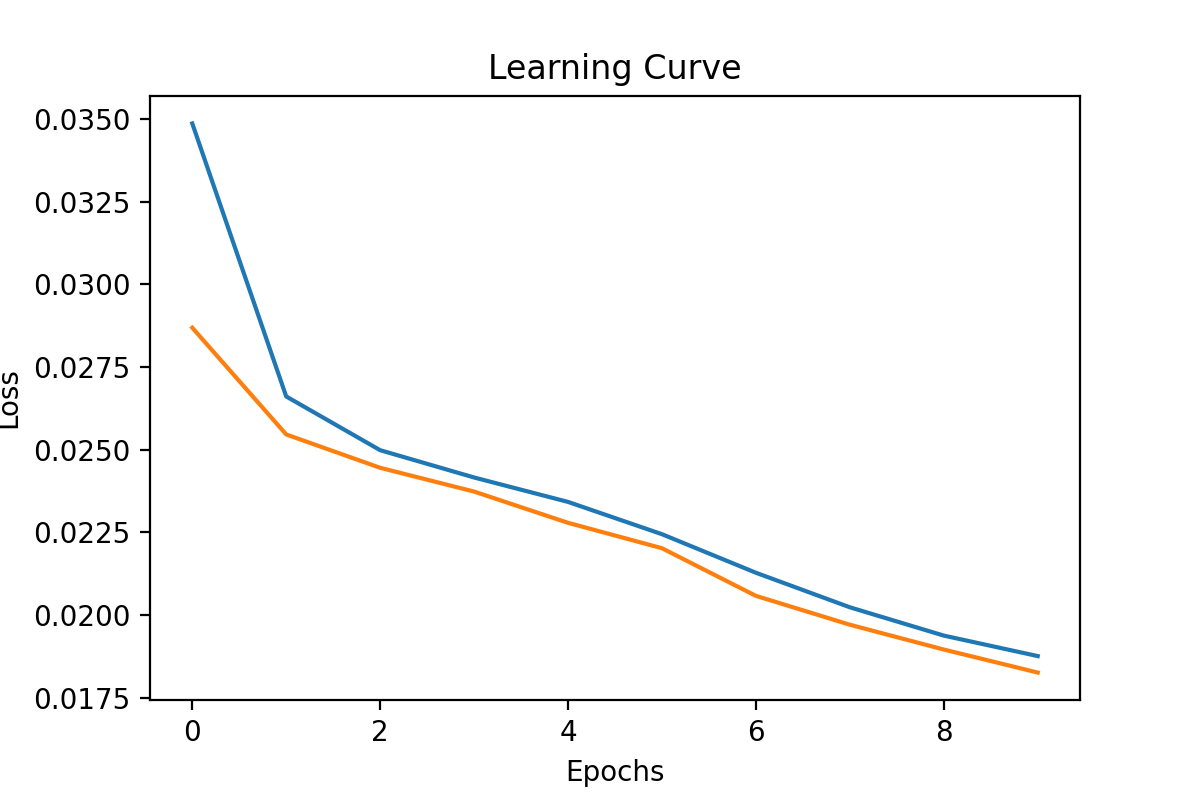
\includegraphics[width=\linewidth]{mlp-learning.png}
  \caption{Learning Curve of MLP Training and Validation Datasets.}
  \label{fig:mlp-learning}
\end{minipage}
\begin{minipage}{0.74\textwidth}
    \centering
    \begin{tabular}{rrrrrrrr}
      \hline
      & Accuracy & Precision & Recall & F1 & F2 & ROCAUC & PRAUC \\
      TS1 & 0.80 & -- & -- & -- & -- & -- & -- \\
      TS2 & 0.91 & 0.00 & 1.00 & 0.00 & 0.00 & 0.99 & 0.00 \\
      TS3 & 0.92 & 0.00 & 0.98 & 0.00 & 0.01 & 0.98 & 0.01 \\
      TS4 & 0.92 & 0.19 & 0.83 & 0.31 & 0.48 & 0.96 & 0.33 \\
      \hline
    \end{tabular}
    \caption{Summary of MLP performance across test sets.}
    \label{tab:mlp-results}
\end{minipage}

\begin{figure}[htb]
  \centering
  \begin{minipage}{0.32\textwidth}
    \centering
    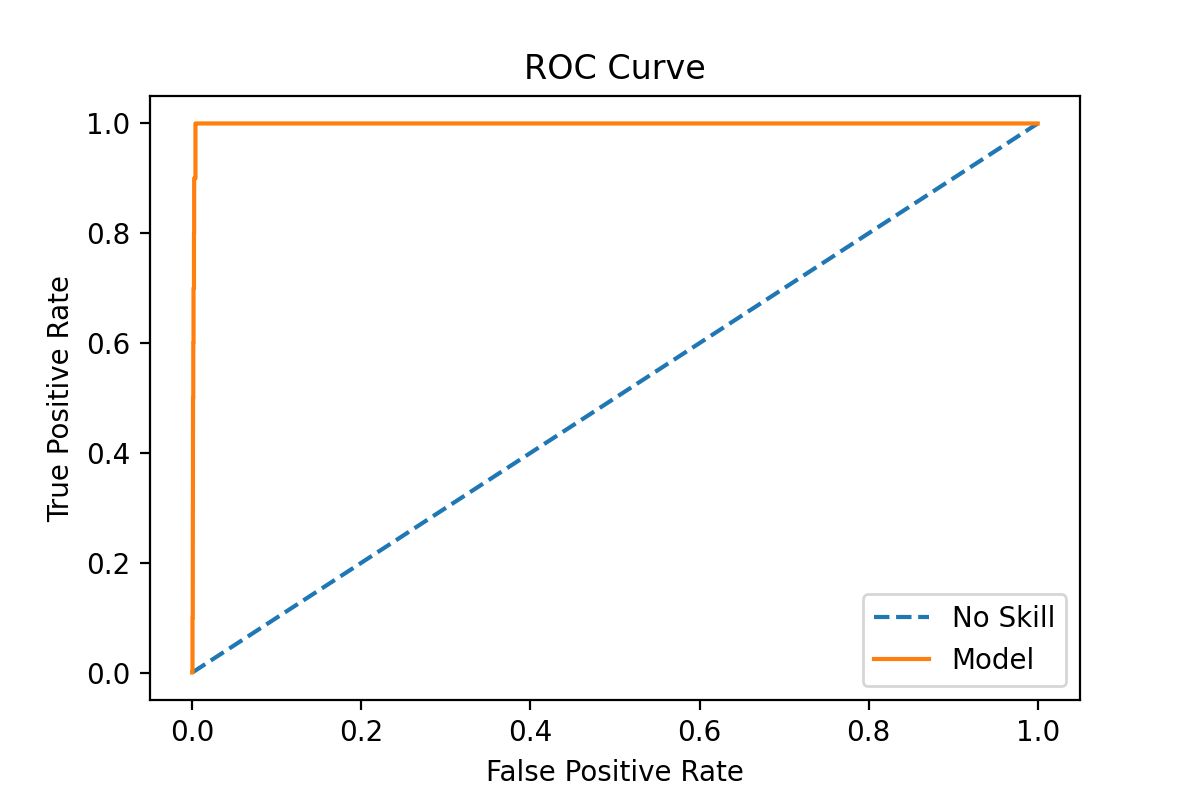
\includegraphics[width=\linewidth]{mlp-roc-low.png}
    \caption{ROC Curve for TS2.}
  \end{minipage}
  \begin{minipage}{0.32\textwidth}
    \centering
    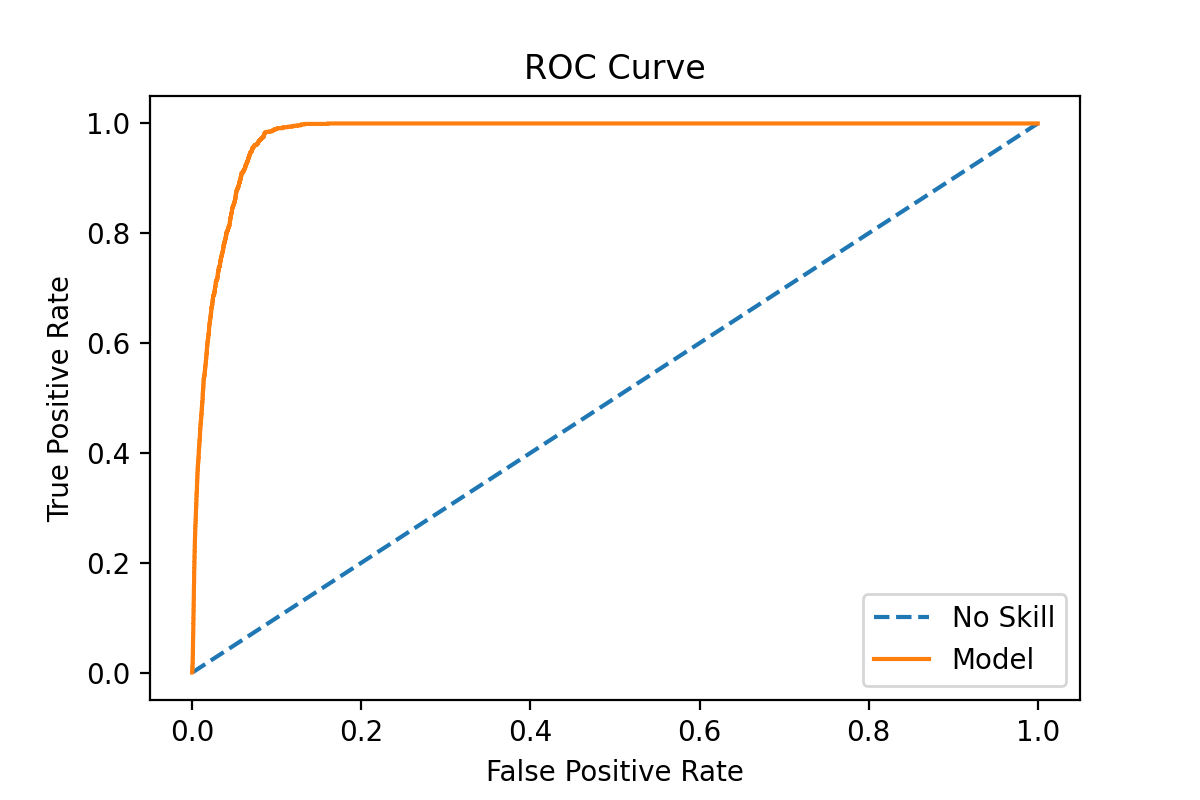
\includegraphics[width=\linewidth]{mlp-roc-medium.png}
    \caption{ROC Curve for TS3.}
  \end{minipage}
  \begin{minipage}{0.32\textwidth}
    \centering
    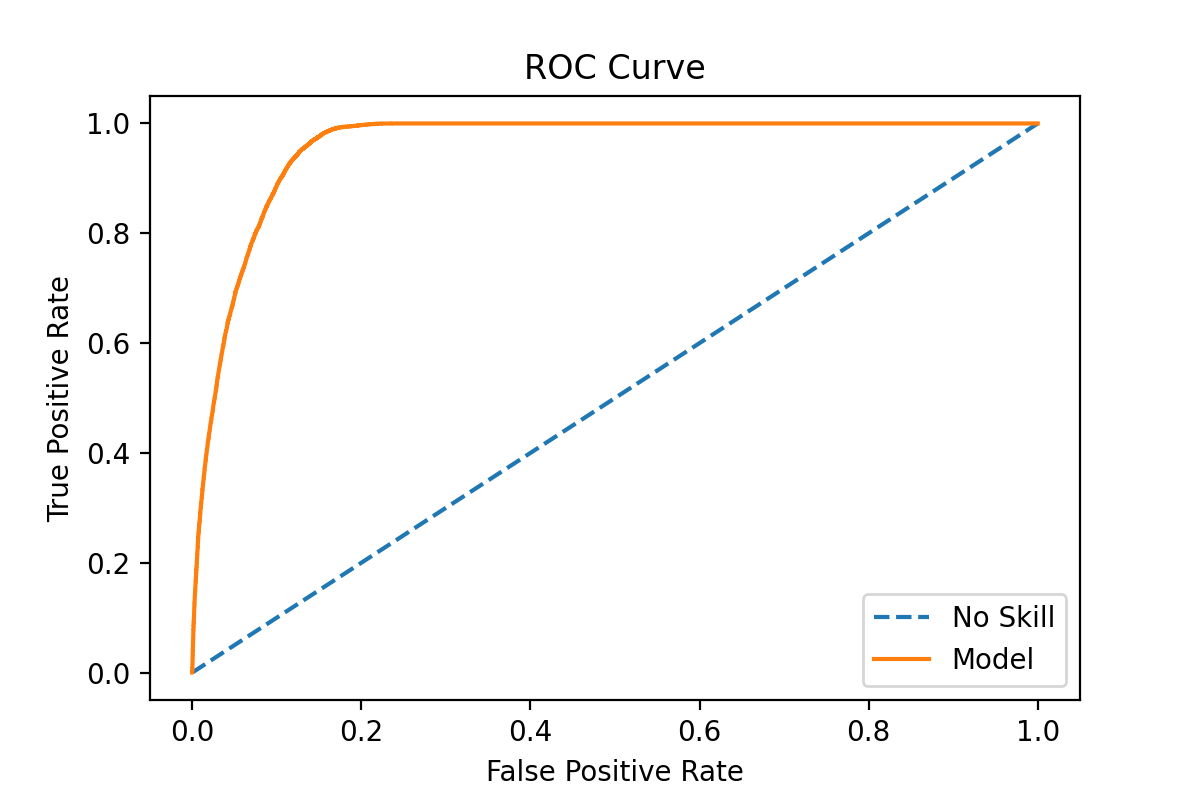
\includegraphics[width=\linewidth]{mlp-roc-high.png}
    \caption{ROC Curve for TS4.}
  \end{minipage}
  \caption{ROC Curves for MLP Test Datasets.}
  \label{fig:mlp-roc}
\end{figure}

The ROC curves paint a different picture (see Figure
\ref{fig:mlp-roc}) with exceedingly high areas. This however is
misleading since ROC curve takes into account the performance for both
the positive and negative classes and thus tend to be overly
optimistic of the model's performance on skewed datasets
\cite{branco2015survey,fernandez2018learning}. In such circumstances,
The PR curves are considered better at gauging a model's skill when
dealing with skewed datasets \cite{branco2015survey}. However, in this
case it too is deemed misleading as it seriously undermines the
model's performance (see Figure \ref{fig:mlp-pr}). This again is
attributed to the precision approaching zero due to the extremely
skewed FP:TP ratio which results in the PRAUC to also be zero.

\begin{figure}[htb]
  \centering
  \begin{minipage}{0.32\textwidth}
    \centering
    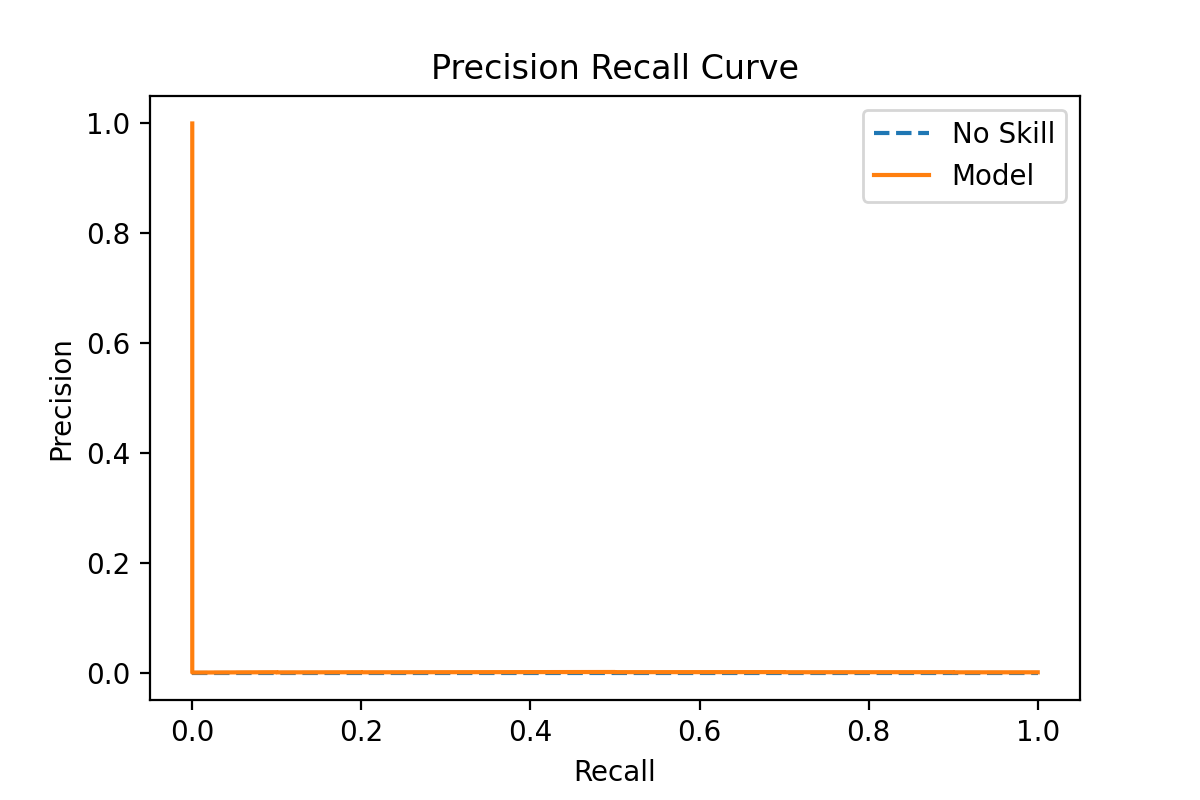
\includegraphics[width=\linewidth]{mlp-pr-low.png}
    \caption{PR Curve for TS2.}
  \end{minipage}
  \begin{minipage}{0.32\textwidth}
    \centering
    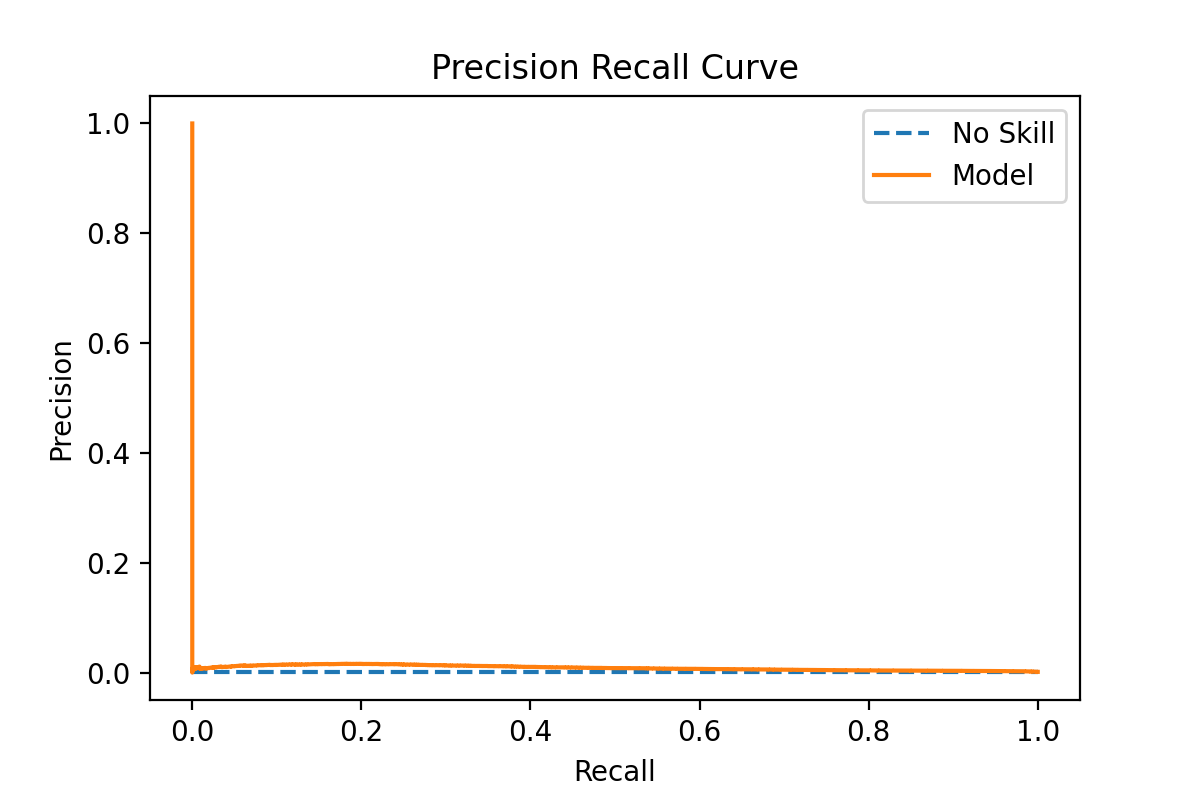
\includegraphics[width=\linewidth]{mlp-pr-medium.png}
    \caption{PR Curve for TS3.}
  \end{minipage}
  \begin{minipage}{0.32\textwidth}
    \centering
    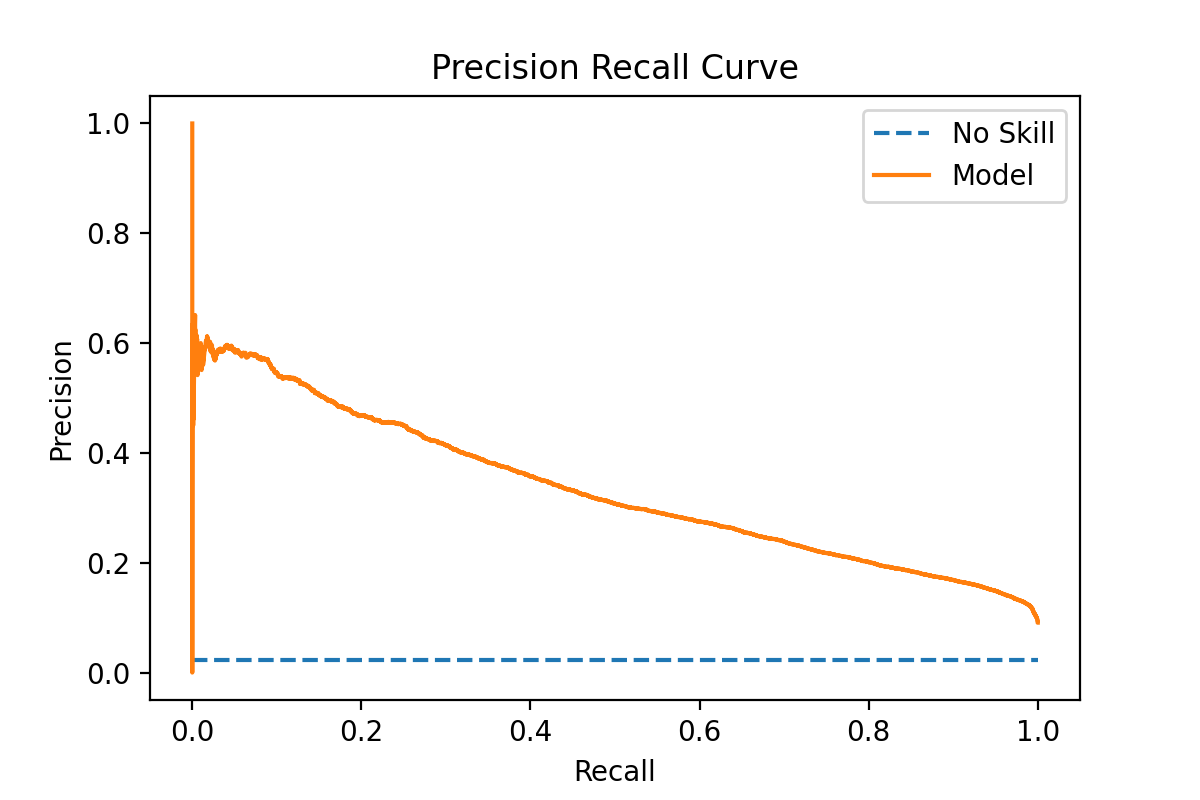
\includegraphics[width=\linewidth]{mlp-pr-high.png}
    \caption{PR Curve for TS4.}
  \end{minipage}
  \caption{PR Curves for MLP Test Datasets.}
  \label{fig:mlp-pr}
\end{figure}

\begin{figure}[htb]
  \centering
  \begin{minipage}{0.32\textwidth}
    \centering
    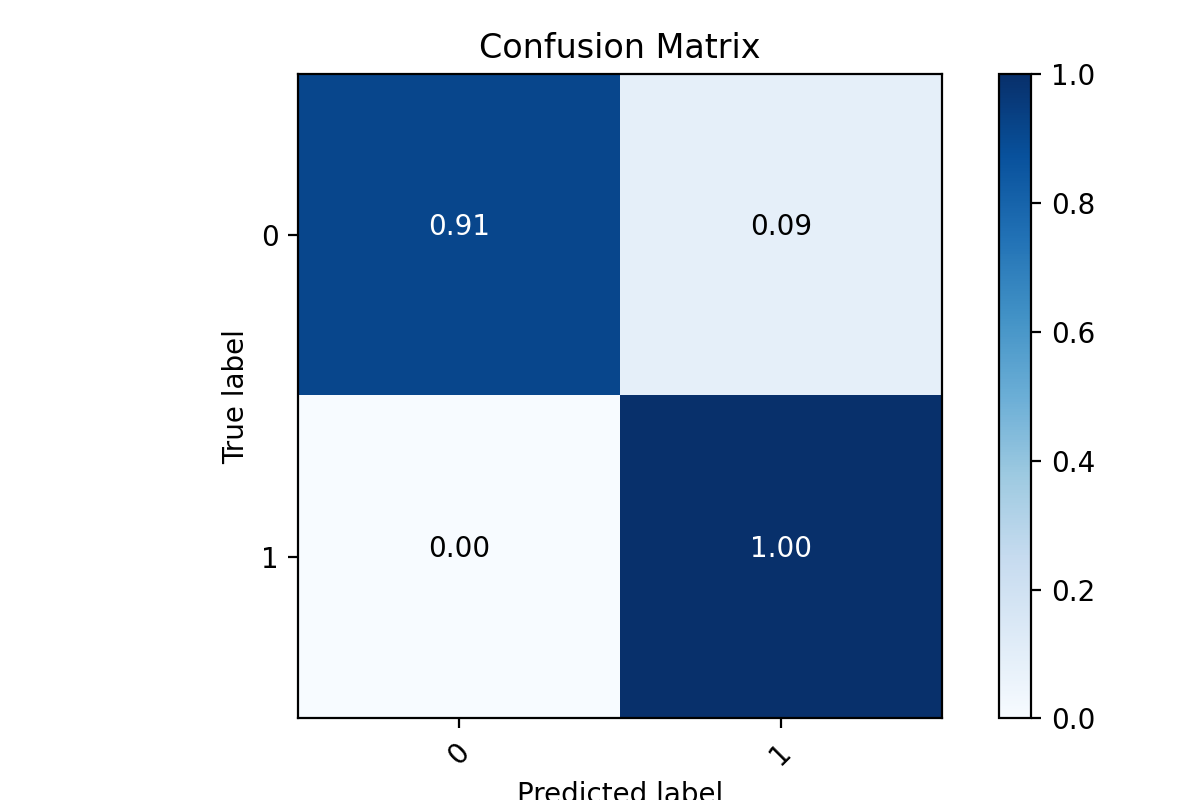
\includegraphics[width=\linewidth]{mlp-cm-norm-low.png}
    \caption{Norm Confusion Matrix for TS2.}
  \end{minipage}
  \begin{minipage}{0.32\textwidth}
    \centering
    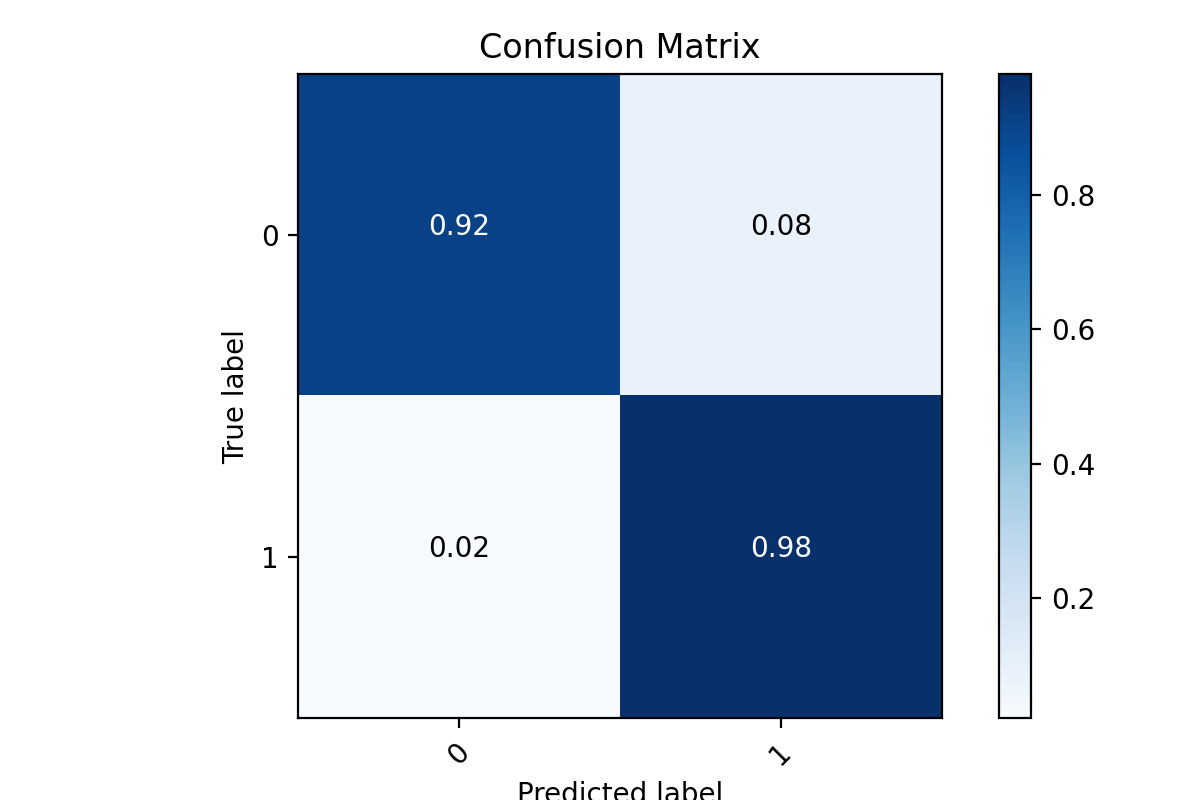
\includegraphics[width=\linewidth]{mlp-cm-norm-medium.png}
    \caption{Norm Confusion Matrix for TS3.}
  \end{minipage}
  \begin{minipage}{0.32\textwidth}
    \centering
    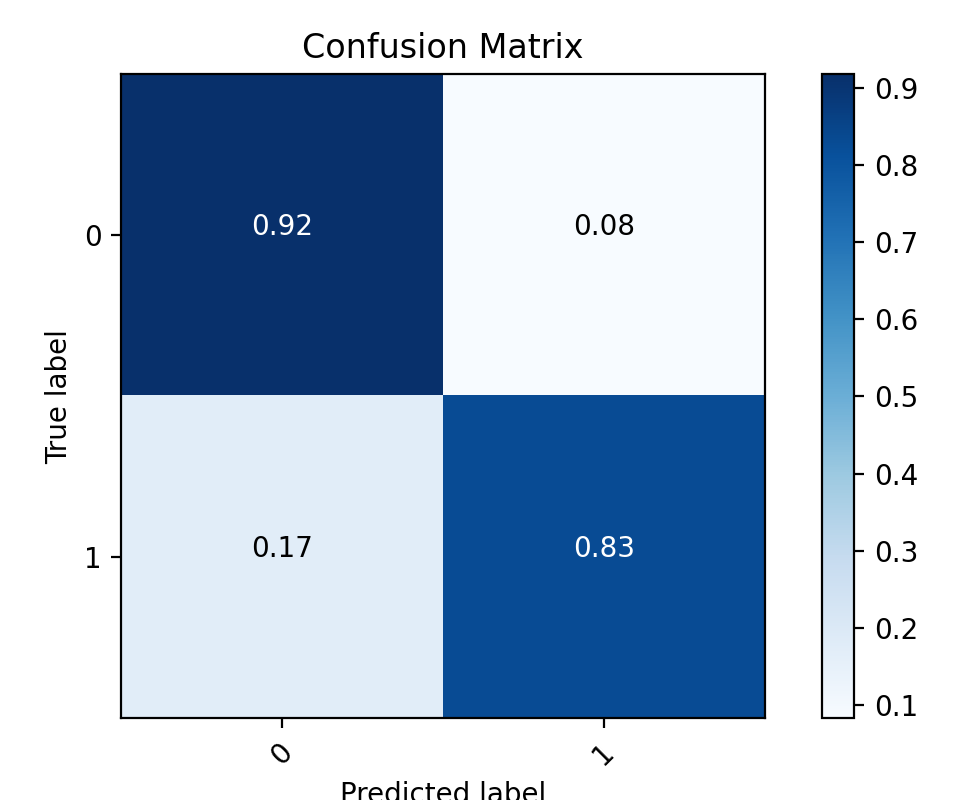
\includegraphics[width=\linewidth]{mlp-cm-norm-high.png}
    \caption{Norm Confusion Matrix for TS4.}
  \end{minipage}
  \caption{Normalized Confusion Matrices of MLP Test Datasets.}
  \label{fig:mlp-cm-norm}
\end{figure}

Figure \ref{fig:mlp-cm} depict the confusion matrices for the various
test datasets. Alternatively, Figure \ref{fig:mlp-cm-norm} can also be
consulted which presents the confusion matrices normalized across the
rows. The confusion matrices highlight the strengths and weaknesses of
the model better than the ROC and PR curves. The model has a very low
number of FNs and FPs which is extremely valuable as this ensures that
the model does not miss hits from neutrino events and also does not
classify hits from noise sources incorrectly as hits from neutrino
events.

\begin{figure}[htb]
  \centering
  \begin{minipage}{0.49\textwidth}
    \centering
    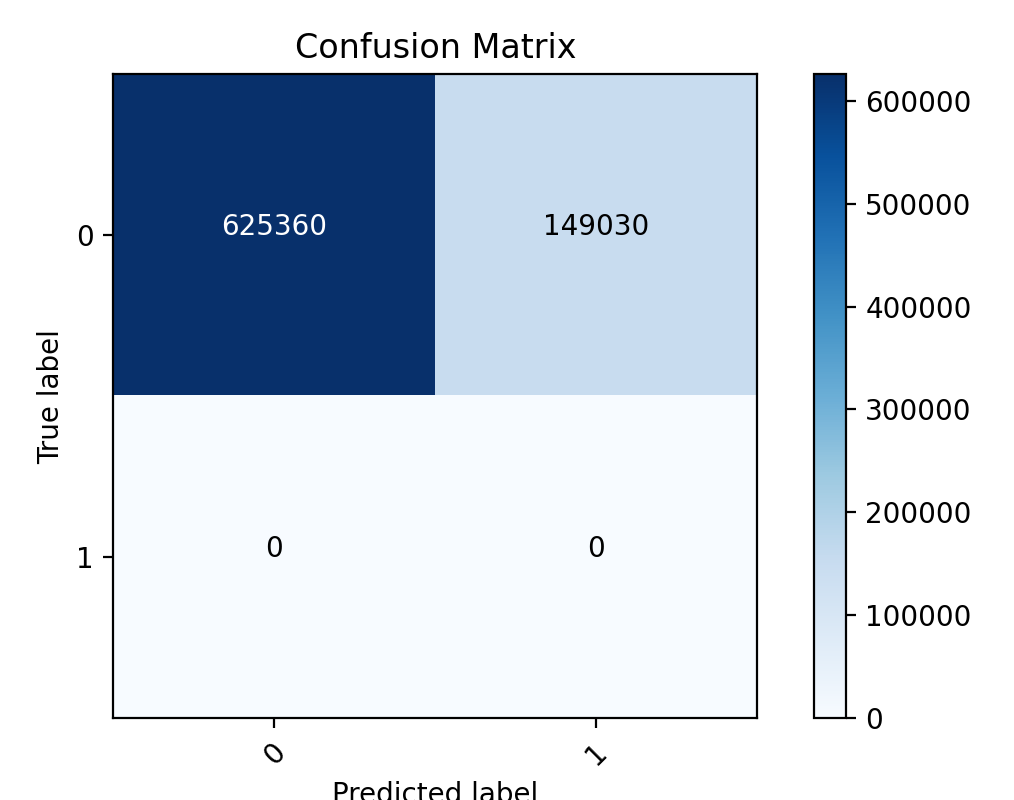
\includegraphics[width=\linewidth]{mlp-cm-no.png}
    \caption{Confusion Matrix for TS1.}
    \label{fig:mlp-cm-no}
  \end{minipage}
  \begin{minipage}{0.49\textwidth}
    \centering
    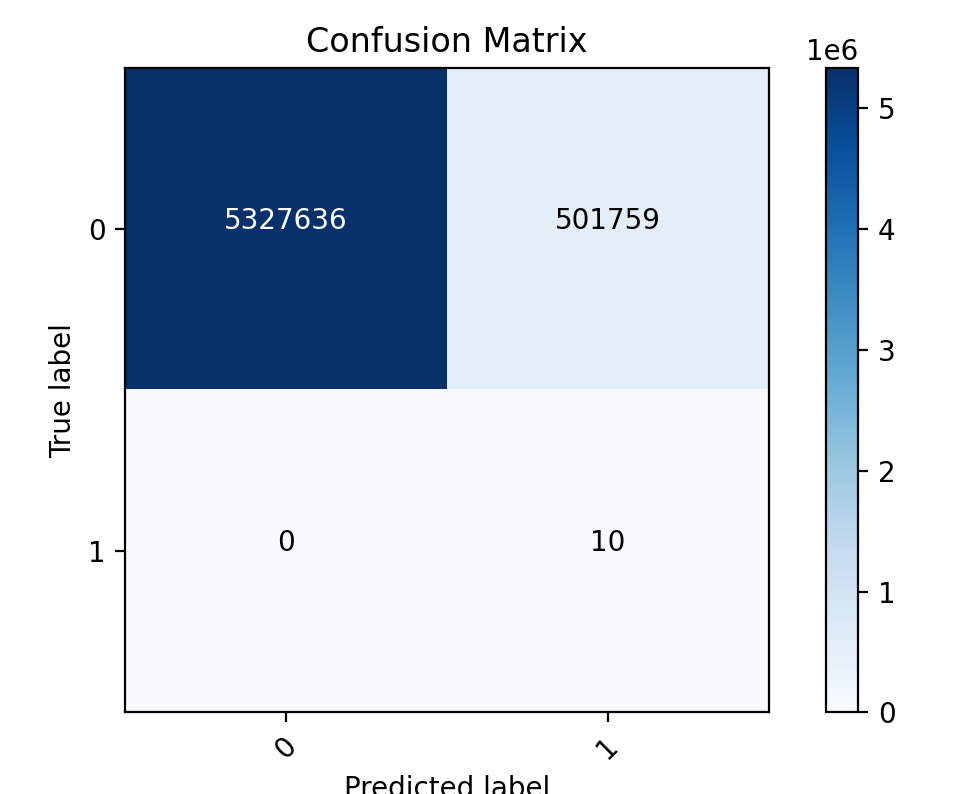
\includegraphics[width=\linewidth]{mlp-cm-low.png}
    \caption{Confusion Matrix for TS2.}
    \label{fig:mlp-cm-low}
  \end{minipage}
  \begin{minipage}{0.49\textwidth}
    \centering
    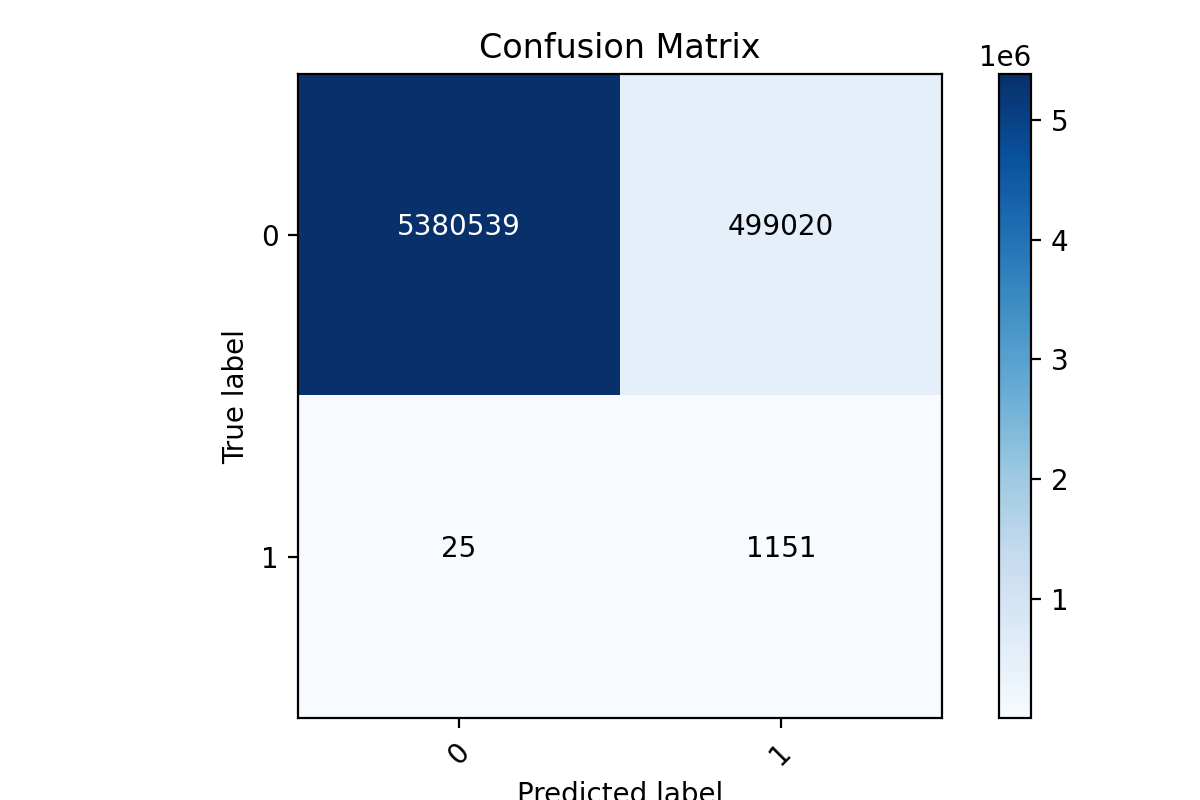
\includegraphics[width=\linewidth]{mlp-cm-medium.png}
    \caption{Confusion Matrix for TS3.}
    \label{fig:mlp-cm-medium}
  \end{minipage}
  \begin{minipage}{0.49\textwidth}
    \centering
    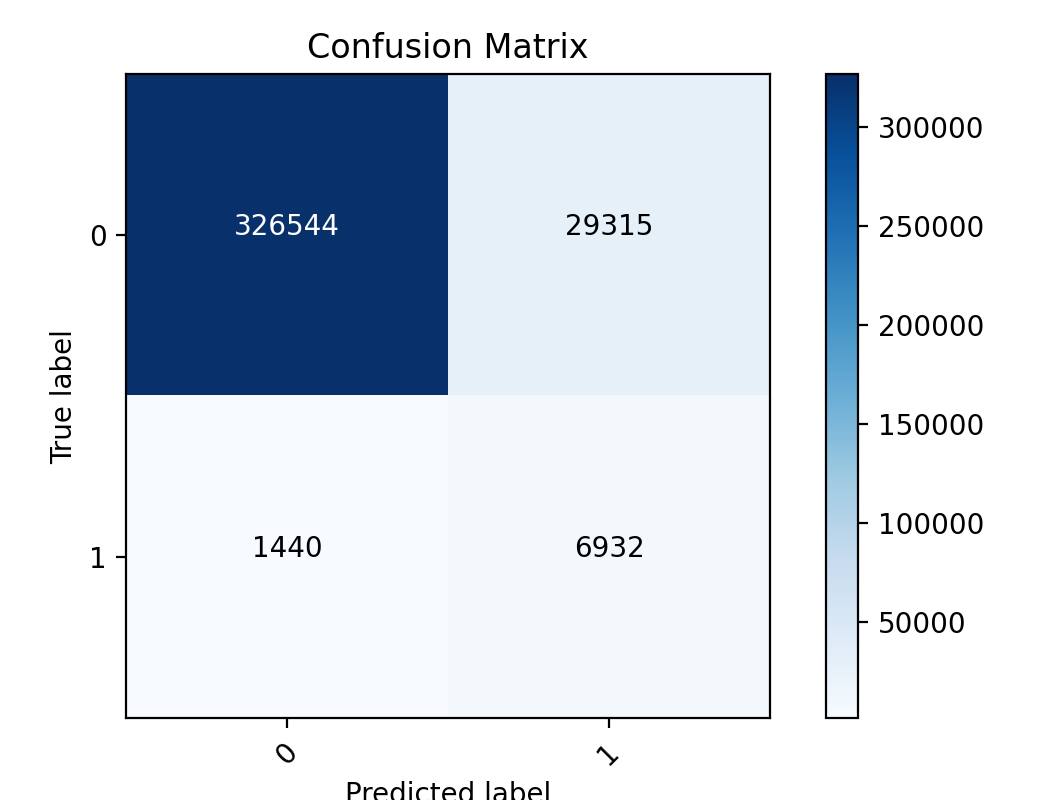
\includegraphics[width=\linewidth]{mlp-cm-high.png}
    \caption{Confusion Matrix for TS4.}
    \label{fig:mlp-cm-high}
  \end{minipage}
  \caption{Confusion Matrices of MLP Test Datasets.}
  \label{fig:mlp-cm}
\end{figure}

% ---------------------------------------------------------------------------
% ----------------------- end of thesis sub-document ------------------------
% ---------------------------------------------------------------------------

% this file is called up by thesis.tex
% content in this file will be fed into the main document

\chapter{Replacement for Graph Community Detection Step} % top level followed by section, subsection
\label{cha:gcn}
% ----------------------- contents from here ------------------------
% 

This chapter presents the replacement created using a Graph
Convolusional Neural Network (GCN) for the \emph{Graph Community Detection
Step} of the Karas pipeline (see \ref{sec:karas-pipeline}). It is
observed that a GCN is able to classify noise and event nodes very
well, even in extremely skewed datasets with less than 10 event nodes.
The chapter begins with an overview of GCNs and how they have been
applied to this problem. The data preparation, visualization and model
evaluation are touched upon next. The chapter concludes with
discussion of the results and next steps.

\section{Primer on Graph Convolusional Neural Networks}
\label{sec:gcn-primer}

\subsection{GNN and graphs}

% TODO mathematical depiction of graphs
GNNs are designed to operate on data which can be represented as
graphs. A graph consists of nodes and edges. Each node may or may not
be connected to one or many nodes, these are referred to as the
neighbors of the node. A graph with all nodes connected to one another
is called a fully connected graph.

An edge may have attributes associated with it, the two most common
attributes being weight and direction. An edge may be directed which
denotes a sense of hierarchy amongst the nodes, or undirected. An edge
may also have a weight to signify a stronger or weaker connection
amongst nodes.

Nodes may also posses attributes associated with themselves, commonly
known as node embeddings. The complexity of the node embedding may
range from a simple scalar quantity to a multi-dimensional tensor,
and depends on the dataset and how the practitioner wishes to sculpt
the graph.

Graphs are primarily classified into two variants.

\begin{enumerate}
\item \textbf{Homogeneous graphs}. Graphs with the same type of nodes
  and edges are referred to as homogeneous graphs. For example, a
  graph representing who follows who on Twitter is a homogeneous
  graph. Here, people are represented as nodes and an edge indicates
  that person A follows person B.
\item \textbf{Heterogeneous graphs}. Graphs with different types of
  nodes and edges are referred to as heterogeneous graphs. For
  example, a graph representing a person's likes and dislikes in
  regards to food items. Here, two entities, namely people and food
  are represented as nodes. The edges also come in two variants ie. a
  'like' and a 'dislike'.
\end{enumerate}
% TODO illustrate types of graphs and their attributes

\subsection{The Message Passing Paradigm}

% TODO illustrate the paradigm
% TODO introduce mathematically?
During each training epoch, a node propagates it's embedding to it's
neighbors and in return receives their embedding. All collected
embeddings are aggregated (for example using a sum, difference or
mean) which becomes the new embedding of the node. This procedure is
done for all nodes of the graph, for each training epoch. The number
of layers in the network determine how far the messages are sent. For
example, for a network with a single layer, each node sends a message
to it's immediate neighbors. With 2 layers, the node also sends a
message to the neighbors of it's immediate neighbors and so forth.

%% \subsection{GNN and it's Variants}

%% GNNs have two primary applications.

%% \begin{enumerate}
%% \item \textbf{Node classification}. This is a semi-supervised learning
%%   setting (although it can also be used in a supervised setting).
%%   Given a graph with nodes associated with a label, the network can be
%%   used to predict the label of unseen nodes.
%% \item \textbf{Graph classification}. In this approach, the network is
%%   trained using several graphs each associated with a label. The
%%   network can then be used to predict the label of an unseen graph.
%% \end{enumerate}


\section{Data Preparation}
\label{sec:gcn-data-prep}

The graphs for the testing and training of the network are constructed
from a combination of the main dataset and a modified version of the
MLP dataset, Figure \ref{fig:gcn-data} illustrates this procedure. A
fully connected graph is constructed, and its node embeddings and node
labels are derived from the main dataset. Thus, each node is thus
assigned a $(x,y,z,t)$ vector as it's node embedding. The node is
assigned a label of 1 if it is an event hit, else a label of 0.

\begin{figure}[h]
  \centering
  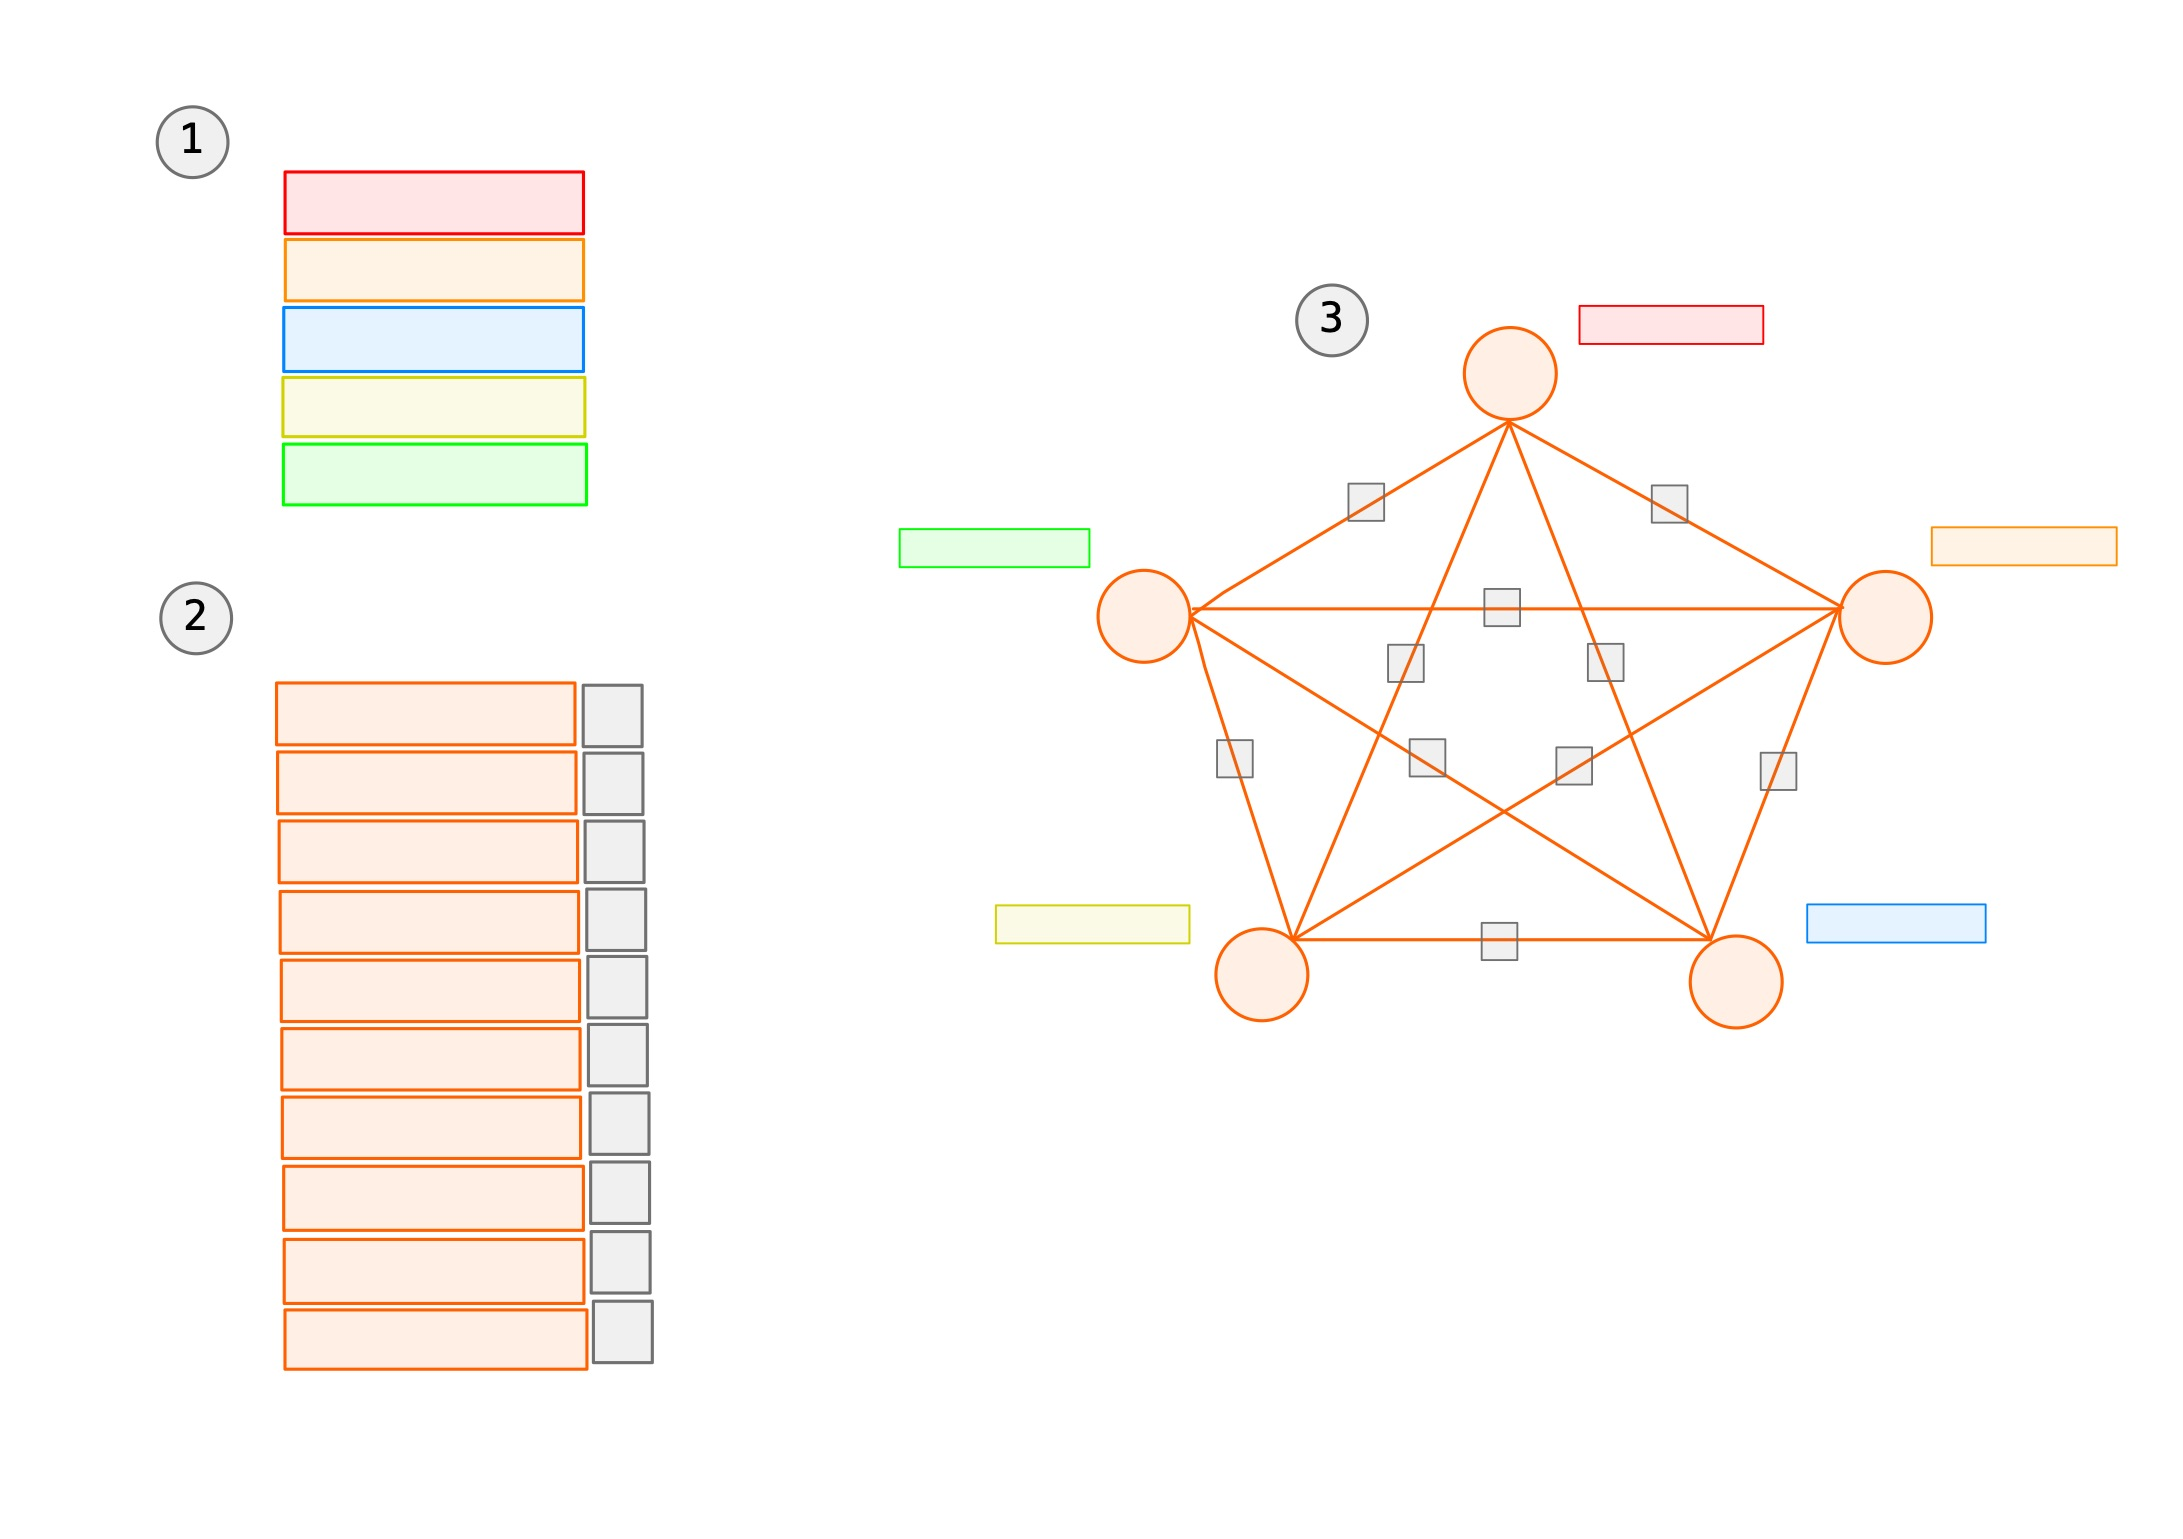
\includegraphics[width=\textwidth]{gcn-data.jpg}
  \caption{Overview of GCN dataset creation procedure. \textbf{(1)} an
    example of the main dataset with 5 hits. \textbf{(2)} the
    corresponding modified MLP dataset created. Although the dataset
    will contain $n^{2}-n = 25$ rows, only the unique rows (10 in this
    example) are shown in the illustration for simplicity.
    \textbf{(3)} The graph representation is created where rows of (1)
    become the node embeddings and the label column of (2) become the
    edge weights.}
  \label{fig:gcn-data}
\end{figure}

A modified MLP dataset (see \ref{sec:mlp-data-prep}) with a shape of
\texttt{$(n^{2}-n, 5)$} is created such that each hit is paired with
all other hits except itself. The label column from this dataset is
then used as the edge weights of the graph. Edges between event nodes
from the same event thus are assigned a weight of 1 and all other
edges are assigned a weight of 0.

%% Data(edge_attr=[999000], edge_index=[2, 999000], x=[1000, 4], y=[1000])
%% Number of nodes: 1000
%% Number of edges: 999000
%% Average node degree: 999.00
%% Edge weight shape: torch.Size([999000])
%% Contains isolated nodes: False
%% Contains self-loops: False
%% Is undirected: True

Since the main dataset and the pattern matrix dataset are highly
skewed, naturally the GCN dataset is also skewed with majority of the
nodes being noise. Similar strategy as used in the creation of the
pattern matrix training set (see \ref{sec:mlp-data-prep}) is
used. The training set is a graph with 1000 nodes equally distributed
amongst the classes.

The skewed nature of the data is maintained in the testing set. The
model is evaluated with 3 test sets each with varying levels of
examples of event nodes. In practise, the pipeline will observe
timeslices with no to very few events thus the performance of the
model on test set 1 and 2 should be given importance.

\begin{enumerate}
\item[\textbf{TS1}.] No event nodes
\item[\textbf{TS2}.] Less than 25 event nodes
\item[\textbf{TS3}.] Less than 250 event nodes
\end{enumerate}

\section{Model Description and Evaluation}
\label{sec:gcn-model-desc-eval}

The model is expected to classify nodes of an unseen graph as event or
noise nodes. Since causally related nodes are connected with edges
carrying a high weight, the model is expected to group them together
thus resulting in a final graph with small clusters of causally
related nodes and a large clusters of noise nodes.

\begin{table}[t]
  \centering
  \begin{tabular}{rr}
    \hline
    Loss & BCELoss \\
    Optimizer & Adam with learning rate of $0.001$ \\
    Hidden Activation & ReLu \\
    Output Activation & Sigmoid \\
    \hline
  \end{tabular}
  \caption{GCN Model Parameter Summary.}
  \label{tab:gcn-model-param}
\end{table}

The parameters of the model are summarized in Table
\ref{tab:gcn-model-param}, the rational for selecting the parameters
being the same as that of the pattern matrix model (see
\ref{sec:mlp-model-desc}) since both models perform binary
classification. The difference comes from the model architecture. The
GCN model comprises of an input layer, two graph convolusional layers
and an output layer. The network is fully connected with 4 neurons in
the input layer, 16 in both graph convolusional layers and 1 neuron in
the output layer.

Evaluation metrics used for evaluating the MLP model are used to
evaluate the GCD model as well (see Section \ref{sec:mlp-model-eval})
since the GCN dataset is also highly skewed in nature.

\section{Discussion}
\label{sec[gcd-disc]}

\begin{table}[htb]
  \begin{tabular}{lrrrrrrr}
    \hline
    & Accuracy & Precision & Recall & F1 & F2 & ROCAUC & PRAUC \\
    \hline
    \multicolumn{8}{c}{Primitive edge weights}
    \hline
    TS1 & TODO & -- & -- & -- & -- & -- & -- \\
    TS2 & 0.58 & 0.04 & 1.00 & 0.08 & 0.18 & 0.87 & 0.06 \\
    TS3 & 0.67 & 0.40 & 1.00 & 0.57 & 0.77 & 0.81 & 0.36 \\
    \hline
    \multicolumn{8}{c}{Advanced edge weights}
    \hline
    TS1 & TODO & -- & -- & -- & -- & -- & -- \\
    TS2 & 1.00 & 1.00 & 1.00 & 1.00 & 1.00 & 1.00 & 1.00 \\
    TS3 & 1.00 & 1.00 & 1.00 & 1.00 & 1.00 & 1.00 & 1.00 \\    
  \end{tabular}
  \caption{Summary of GCN performance across test sets.}
  \label{tab:gcn-results}
\end{table}

% ---------------------------------------------------------------------------
% ----------------------- end of thesis sub-document ------------------------
% ---------------------------------------------------------------------------

% this file is called up by thesis.tex
% content in this file will be fed into the main document

\chapter{Recommendations} % top level followed by section, subsection
\label{cha:rec}

% ----------------------- contents from here ------------------------
%

This chapter presents some practical recommendations for the readers
who wish to use the new data processing pipeline presented in this
report. The chapter also presents alternative paths of research which
remain unexplored and general improvements that can be made to the
pipeline in the future.

The Multi Layered Perceptron presented in Chapter \ref{cha:mlp}
capable of identifying causally related hits with a higher accuracy,
precision and recall compared to the Pattern Matrix Criterion
presented by Karas et al. and thus is considered a viable successor to
the PMC. Although experiments were done to identify the optimal
parameters such as the batch size, optimization function, learning
rate, height and depth of the network, further experimentation is
recommended before it is integrated into the Data Acquisition
Pipeline. The model also showed an increase in the number of FPs when
the number of positive class examples are increased. It may be
possible to correct this bias by adding some regularization into the
model \cite{Goodfellow-et-al-2016}.

\begin{table}[htb]
  \centering
  \caption{Advanced edge weight scheme for GCN.}
  \begin{tabular}{lr}
    \hline
    Node type(s) & Edge weight \\
    \hline
    noise-noise & 1.0 \\
    event-event (causally related) & 1.0 \\
    event-event (causally unrelated) & 0.5 \\
    event-noise & 0.1 \\
    \hline
  \end{tabular}
  \label{tab:gcn-adv-weights}
\end{table}

The GCN obtained in Chapter \ref{cha:gcn} has a perfect recall however
is also significantly biased to the positive class (event nodes) and
thus unable to identify the negative class (noise nodes). The origin
of the problem can be traced back to the edge weights being applied to
the graph. The weights supplied by the MLP only take into account
edges between causally related and unrelated hits. In reality however,
unrelated hits consists of various sub categories: 1. noise-noise hits
2. noise-event hits and 3. causally unrelated event-event hits.
Although from a physics point of view the pairs of hits listed above
are in fact causally unrelated, this \emph{naive} edge weight scheme
does not allow the GCN to learn adequately. The root cause of this
conflict is based in the fact that the two models have contradictory
goals. Whilst the MLP is trained to identify causally related and
unrelated hits, the GCN is required to identify hits originating from
neutrino events and noise. The solution is simple and requires
assigning edge weights based on the nodes that it connects as
summarized in Table \ref{tab:gcn-adv-weights}. The GCN model is
trained using the \emph{advanced} edge weight scheme and the results
are promising as observed in Figure \ref{fig:gcn-cm-adv} and
\ref{fig:gcn-test-tsne-adv}. The model now has perfect discriminatory
skills for both classes even in the extremely skewed datasets like
TS2.

\begin{figure}[htb]
  \begin{minipage}{0.32\textwidth}
    \centering
    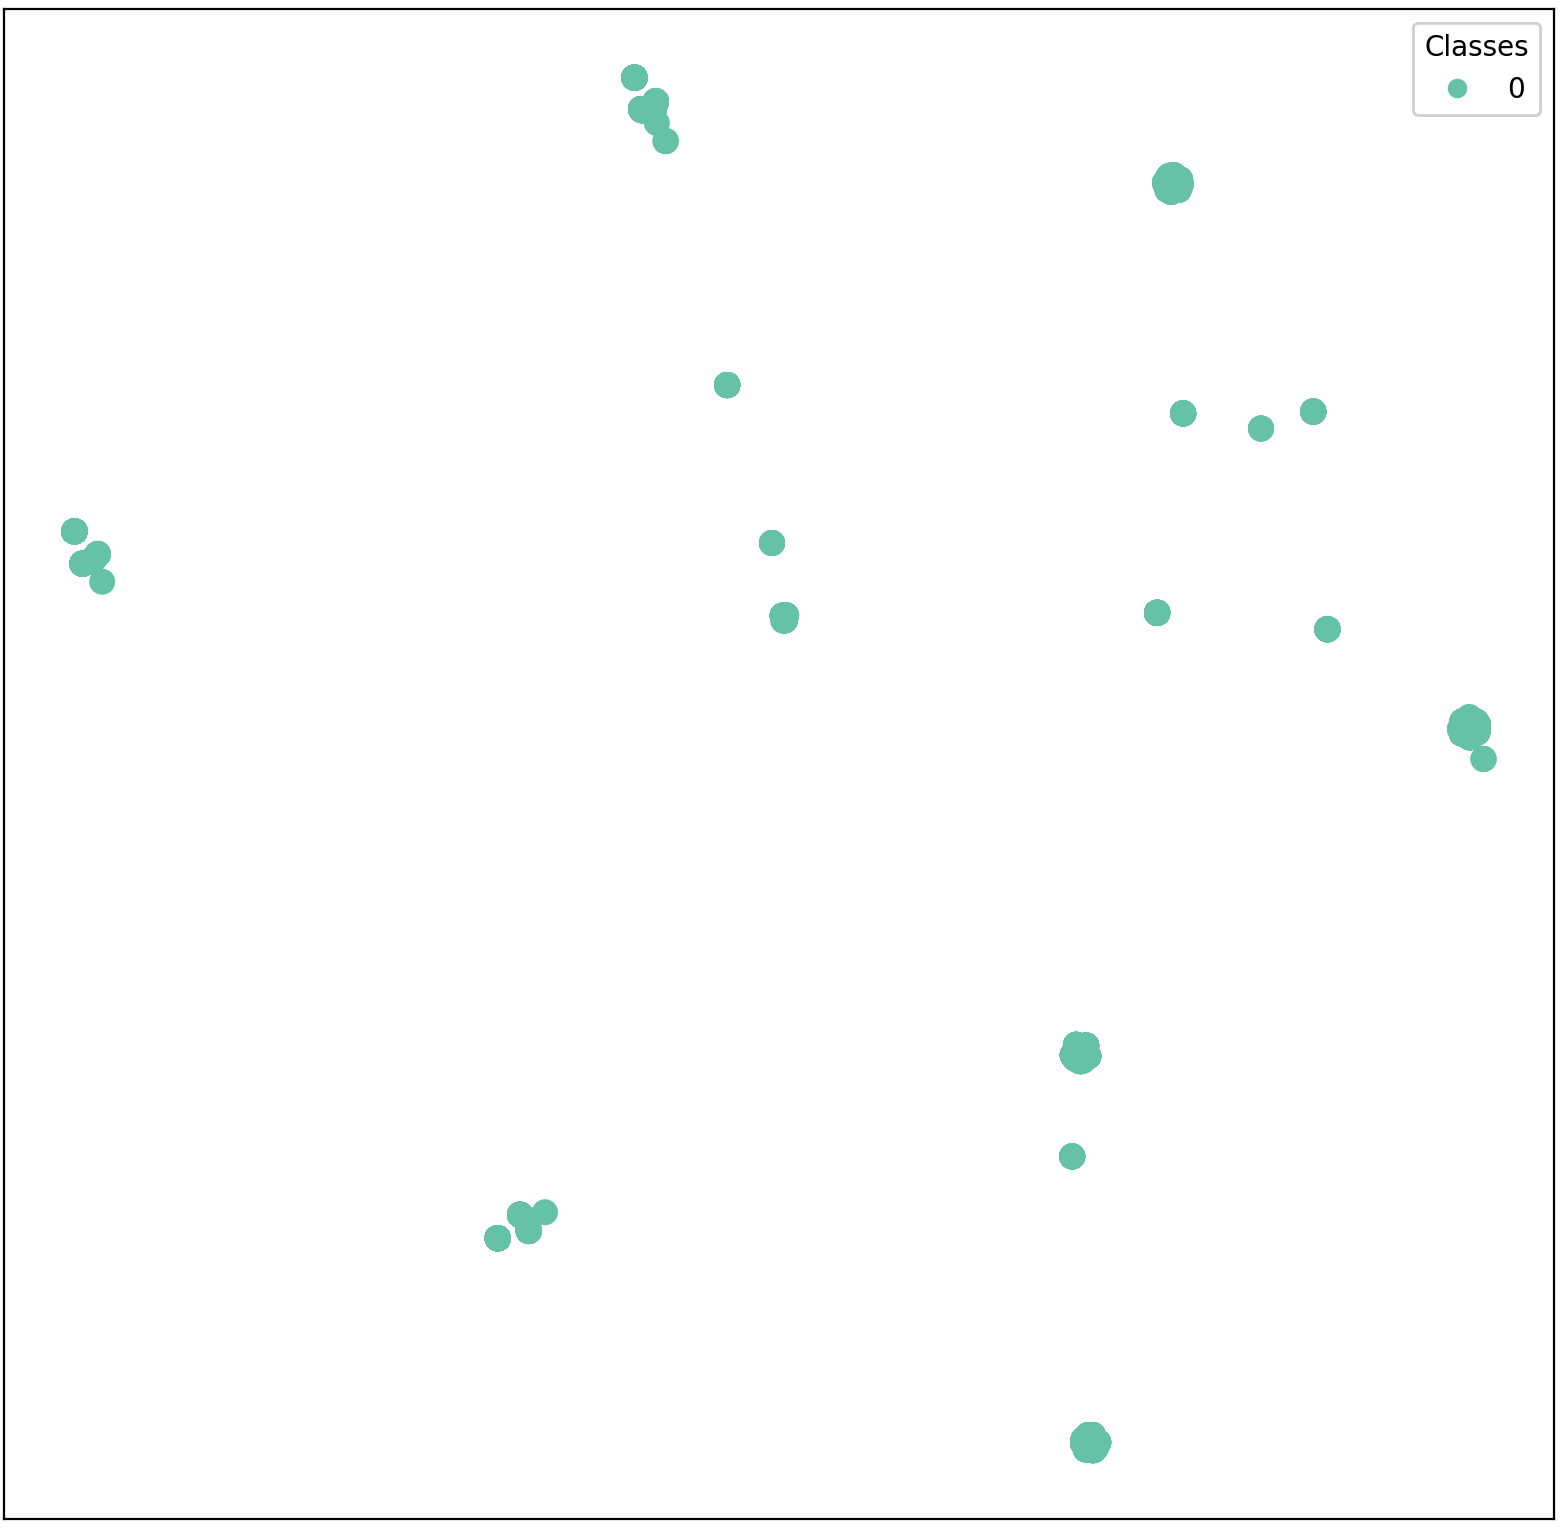
\includegraphics[width=\linewidth]{gcd-adv-test-no-tsne-after.png}
    \caption{TSNE for TS1 with advanced edge weights.}
  \end{minipage}
  \begin{minipage}{0.32\textwidth}
    \centering
    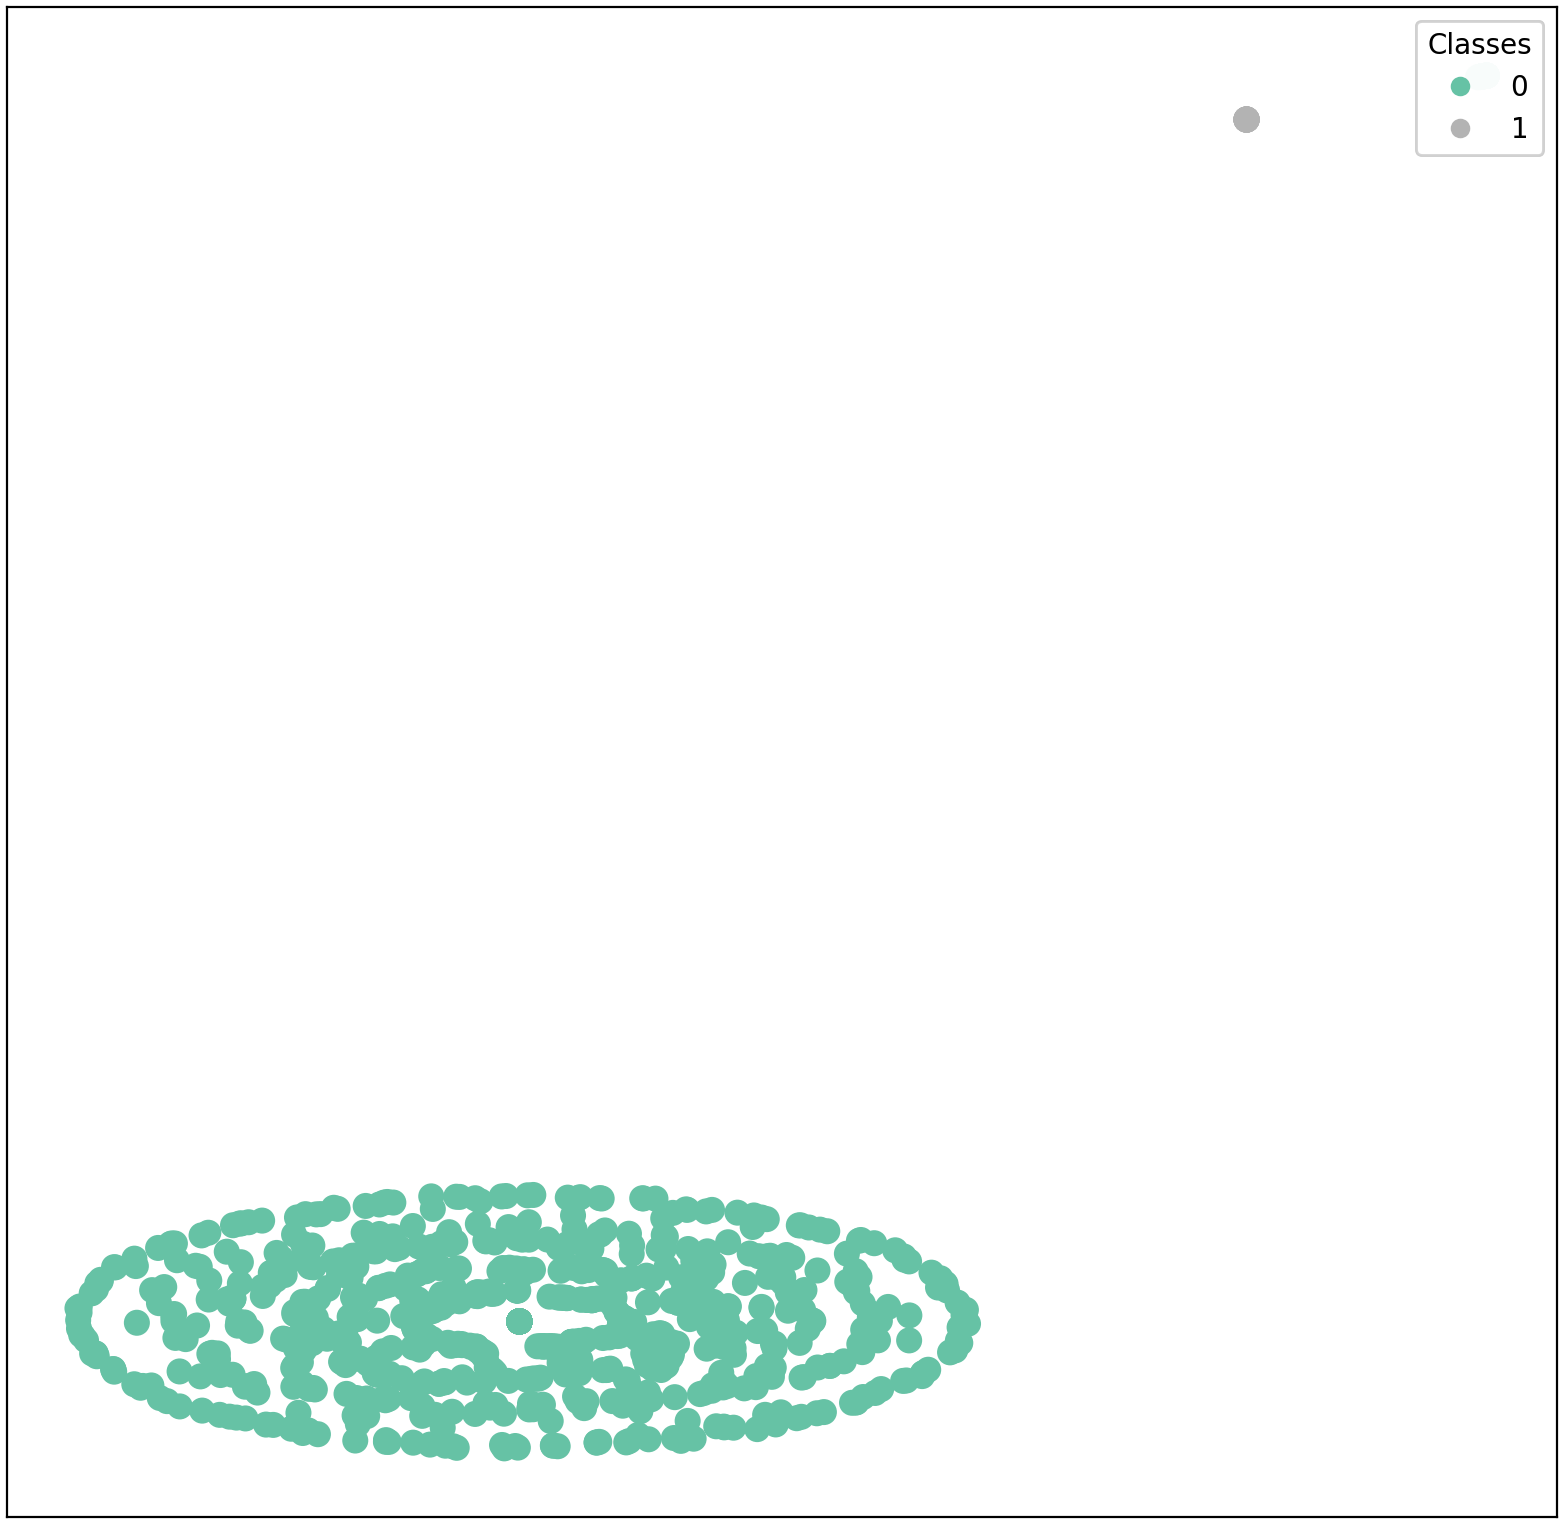
\includegraphics[width=\linewidth]{gcd-adv-test-medium-tsne-after.png}
    \caption{TSNE for TS2 with advanced edge weights.}
  \end{minipage}
  \begin{minipage}{0.32\textwidth}
    \centering
    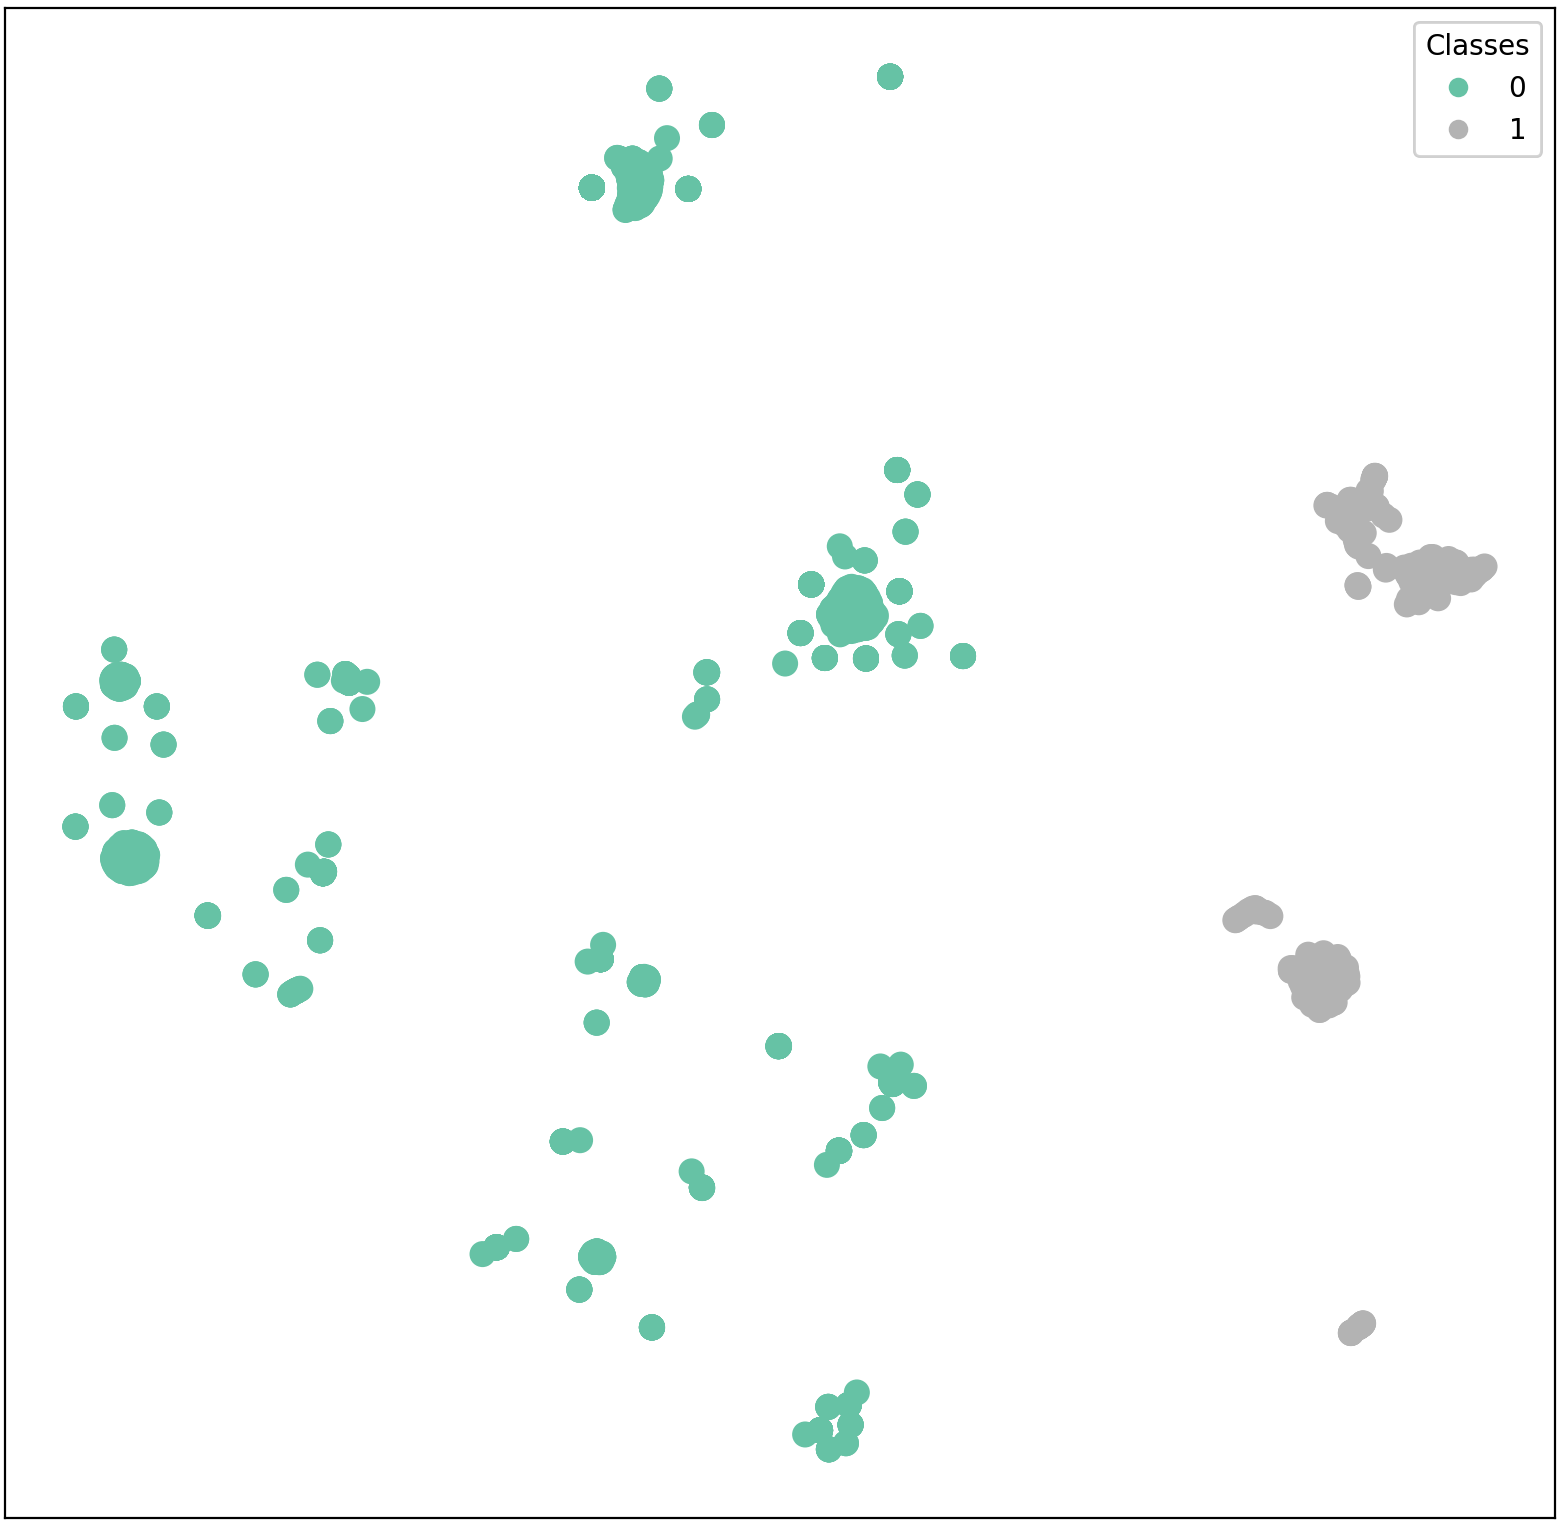
\includegraphics[width=\linewidth]{gcd-adv-test-high-tsne-after.png}
    \caption{TSNE for TS3 advanced edge weights.}
  \end{minipage}
  \caption{TSNE for GCN test datasets with advanced edge weights.}
  \label{fig:gcn-test-tsne-adv}
\end{figure}

\begin{figure}[htb]
  \centering
    \begin{minipage}{0.32\textwidth}
    \centering
    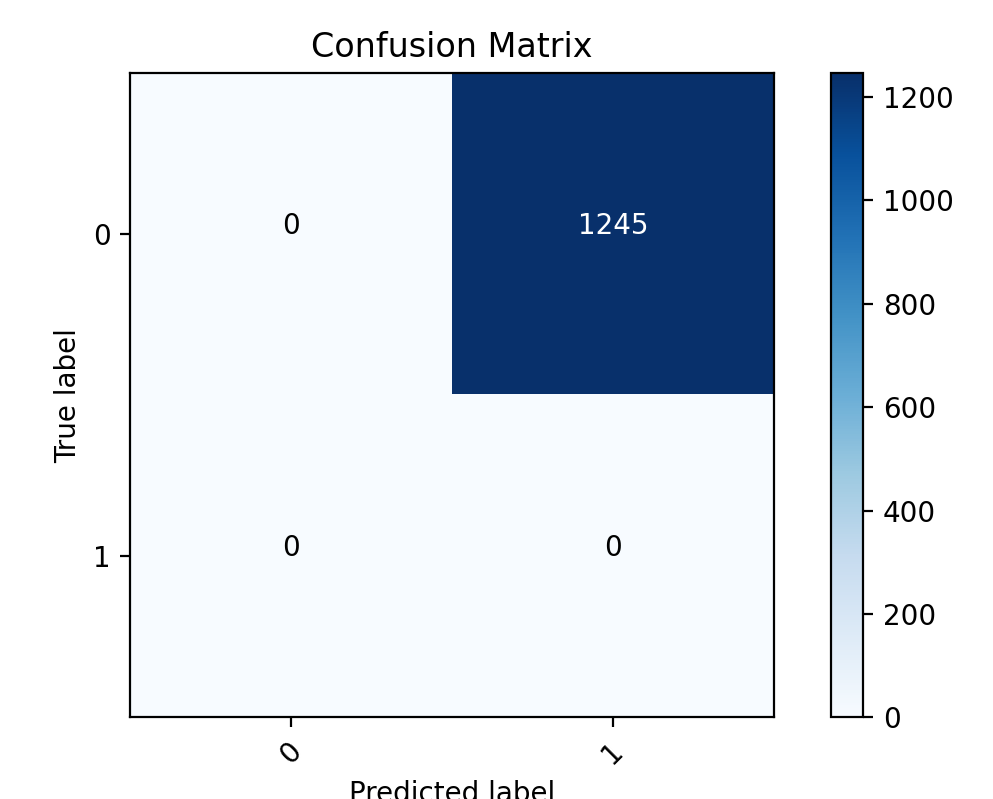
\includegraphics[width=\linewidth]{gcd-adv-cm-no.png}
    \caption{CM for TS1 (advanced edge weights).}
  \end{minipage}
  \begin{minipage}{0.32\textwidth}
    \centering
    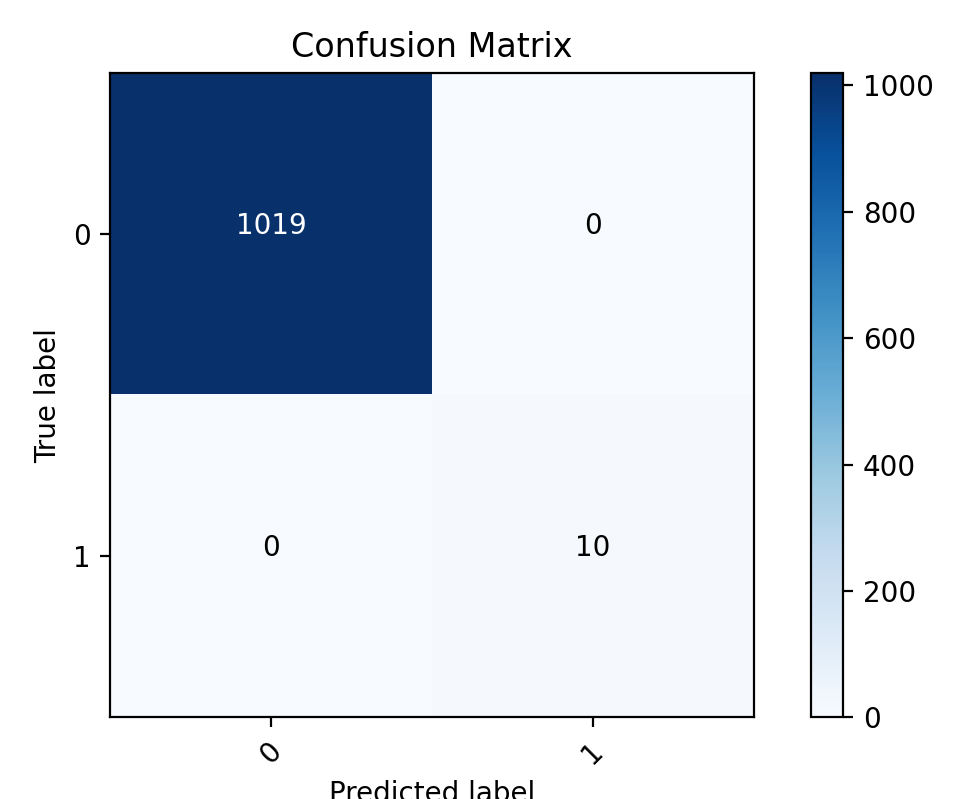
\includegraphics[width=\linewidth]{gcd-adv-cm-medium.png}
    \caption{CM for TS2 (advanced edge weights).}
  \end{minipage}
  \begin{minipage}{0.32\textwidth}
    \centering
    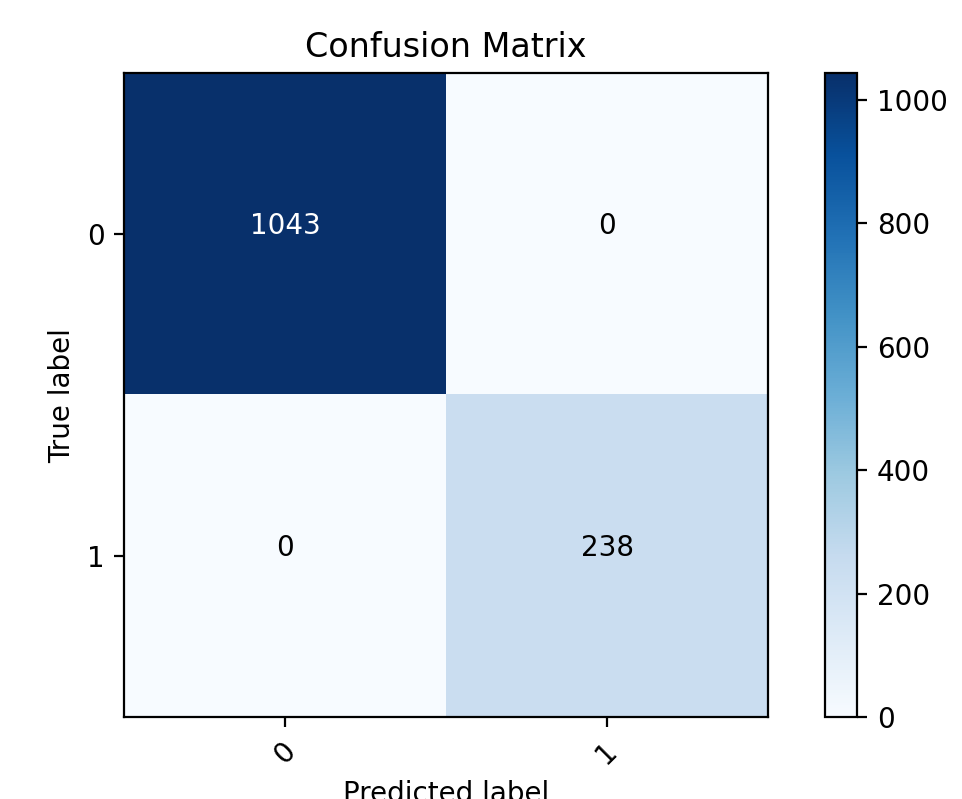
\includegraphics[width=\linewidth]{gcd-adv-cm-high.png}
    \caption{CM for TS3 (advanced edge weights).}
  \end{minipage}
  \caption{CM for GCN test datasets with advanced edge weights.}
  \label{fig:gcn-cm-adv}
\end{figure}

Although the GCN is now capable of identifying event and noise nodes
with immaculate accuracy, precision and recall, it however classifies
all examples as false positives in TS1 which contains no event nodes.
The model is thrown off by the high weights on edges between causally
related event nodes and noise nodes, which may be possible correct by
framing the data as a multi-edge heterogeneous graph. By creating
different types of edges corresponding to the various types of
connections that two nodes may posses, each carrying the corresponding
weights, the network may be able to correct it's bias to the positive
class. In order to obtain the advanced edge weight, the MLP must be
modified such that it performs multi-class classification on the edge
types. For a classification problem of n edge types, the output of the
MLP will thus become a \texttt{(n,)} vector containing the expected
probability for each class. These probabilities can then be used as
the edge weights as illustrated in Figure \ref{fig:gcn-hetero}. The
MLP may not be able to discern causally unrelated hits since they are
spread evenly in space and time, thus research to identify an
appropriate model for the task is required. One approach may be to use
a GCN to perform classification of the edge types or regression on the
edge weights \cite{gong2019exploiting} however this remains to be
validated.
% TODO illustrate heterogeneous graph approach

\begin{table}[htb]
  \centering
  \caption{Summary of GCN performance across test sets with advanced
    edge weights.}
  \begin{tabular}{lrrrrrrr}
    \hline
    & Accuracy & Precision & Recall & F1 & F2 & ROCAUC & PRAUC \\
    \hline
    TS1 & 0.00 & -- & -- & -- & -- & -- & -- \\
    TS2 & 1.00 & 1.00 & 1.00 & 1.00 & 1.00 & 1.00 & 1.00 \\
    TS3 & 1.00 & 1.00 & 1.00 & 1.00 & 1.00 & 1.00 & 1.00 \\
    \hline
  \end{tabular}
  \label{tab:gcn-results-adv}
\end{table}

We observed a high coupling of the Hit Correlation Step with the
subsequent steps of the Karas Pipeline. The output of the PMC is used
by the steps that follow so any shortcomings of the PMC cascade down
the pipeline and affect the performance of the latter steps and the
pipeline as a whole. This coupling is also present in the new pipeline
as the performance of the MLP directly dictates the performance of the
GCN. This coupling is not ideal and an effective solution to decouple
the two models is required. One such solution which remains open as a
path of research is to explore the possibility of replacing the entire
pipeline with a single GCN. The data can be framed such that the $(x,
y, z)$ vectors are used as the node embedding. If the \emph{t} is
scaled between $[0, 1]$ and the complement of $\delta t$ is assigned
as the edge weights, it should result in a graph where edges between
causally related nodes carry a high weight. After convolusion, a
reasonable expectation is the presence of small and tightly connected
communities of causally related nodes and large, weakly connected
communities of noise nodes. The GCN model can now be modified to
perform graph classification \cite{zhang2018end} instead of node
classification, the premise being that presence of small, densely
connected communities indicate the timeslice is important and thus
should be saved for further analysis. Alternatively, the Line Graph
Neural Network proposed by Chen et al. (2017) can also be used to
perform community detection.

The models presented in this report were tested in isolation. The
intended usage however is to use them in tandem in order to identify
timeslices containing neutrino event hits. Thus it is recommended that
the models be tested as an integrated pipeline so that the results may
be compared to that of The Karas Pipeline. Additionally, performance
of the pipeline should be observed using various permutations of the
individual parts of the new and the old pipeline to determine the best
performing combination overall. As noted in Section
\ref{sec:user-req}, the runtime performance of the pipeline is crucial
and should be able to perform filtration in near real time. As neural
networks can be parallelized using the compute power of GPUs, the
models should be capable of meeting the requirements. Several existing
work also indicate the feasibility of scaling GCNs to parallel
computation over large graphs \cite{ma2019high, ma2019neugraph,
  zeng2019accurate}, however the data preparation may pose a
bottleneck. Of course at this point these are merely speculations and
empirical proof still requires to be gathered.

% ---------------------------------------------------------------------------
% ----------------------- end of thesis sub-document ------------------------
% ---------------------------------------------------------------------------


%% this file is called up by thesis.tex
% content in this file will be fed into the main document

\chapter{Conclusion} % top level followed by section, subsection

% ----------------------- contents from here ------------------------
% 

This report presented the research undertaken to validate the
application of Deep Learning for neutrino detection in the KM3NeT
Neutrino Telescope. Chapter \ref{cha:intro} presented an introduction
to the problem space and its importance, the stakeholders and their
requirements and finally the research questions this project sought to
answer. In Chapter \ref{cha:data}
% ---------------------------------------------------------------------------
% ----------------------- end of thesis sub-document ------------------------
% ---------------------------------------------------------------------------


%% this file is called up by thesis.tex
% content in this file will be fed into the main document

%: ----------------------- name of chapter  -------------------------
\chapter*{Appendix} % top level followed by section, subsection


%: ----------------------- paths to graphics ------------------------

% change according to folder and file names
\ifpdf
    \graphicspath{{X/figures/PNG/}{X/figures/PDF/}{X/figures/}}
\else
    \graphicspath{{X/figures/EPS/}{X/figures/}}
\fi

%: ----------------------- contents from here ------------------------
\includepdf[pages=1-5]{CodesTable} 
\includepdf[pages=1-4]{InterviewQuestions}





% ---------------------------------------------------------------------------
%: ----------------------- end of thesis sub-document ------------------------
% ---------------------------------------------------------------------------




% --------------------------------------------------------------
%:                  BACK MATTER: appendices, refs,..
% --------------------------------------------------------------

% the back matter: appendix and references close the thesis


\bibliography{references} % adjust this to fit your BibTex file

% according to Dresden med fac summary has to be at the end
%
% Thesis Abstract -----------------------------------------------------


%\begin{abstractslong}    %uncommenting this line, gives a different abstract heading
\begin{abstracts}        %this creates the heading for the abstract page

  Neutrinos are highly elusive subatomic particles which can only be
  detected with the help of large particle detectors. The KM3NeT
  neutrino telescope is one such detector currently being constructed
  at the bottom on the Mediterranean Sea. Due to its large volume and
  the presence of background noise, ``event trigger'' algorithms are
  utilized by the data acquisition pipeline of the detector to sift
  through the noise. A GPU Pipeline was also developed to improve the
  quality of filtration of the event trigger algorithms without
  compromising their runtime performance. Despite these efforts, the
  quality of filtration require further improvements. The goal of this
  paper is to improve upon the GPU Pipeline using Artificial Neural
  Networks. The paper explores the possibility of replacing parts of
  the GPU Pipeline using Multi Layer Perceptrons and Graph
  Convolutional Neural Networks. The Multi Layer Perception performs
  better compared to the existing solution while the results of the
  Graph Convolutional Network are inconclusive in its existing form.
  Overall, the outcome is promising and new avenues of research are
  discovered through this work.

  \emph{\textbf{Keywords}: Neutrino detection, Artificial Neural
  Network, Multi Layer Perception, Deep learning, Graph Neural
  Networks, Geometric Learning, KM3NeT.}
\end{abstracts}
%\end{abstractlongs}


% ---------------------------------------------------------------------- 


%: Declaration of originality
%\include{8_backmatter/declaration}



\end{document}
